\chapter{Modelling}

% Required packages in the preamble:
% \usepackage{graphicx}
% \usepackage{booktabs}
% \usepackage{float}

\section{Baseline Models and Initial Explainability Analysis}
\label{sec:baselines}

Two baseline configurations were established before evaluating more advanced
approaches such as data augmentation and transfer learning. The objective was
not only to obtain reference classification performance, but also to examine
whether the convolutional neural network (CNN) relied on non-pulmonary or
dataset-specific visual cues.

The first baseline used the complete chest radiograph and represented an
unconstrained classification setting. However, additional region-based
experiments showed that substantial predictive information was also present
outside the segmented lung fields. Therefore, a second baseline was introduced
using a lung-centred region of interest (ROI). In this configuration, the lung
segmentation masks were used only to localise the thoracic ROI and were not
applied directly to the input image. This avoided the artificial black
boundaries introduced by hard lung masking while reducing peripheral image
content.

The two baselines therefore served complementary purposes:

\begin{itemize}
    \item \textbf{Full-image baseline:} measures the classification performance
    achievable from the complete chest X-ray.
    \item \textbf{Lung-ROI baseline:} provides a more spatially controlled
    reference in which peripheral image regions are reduced while the original
    radiographic appearance is preserved.
\end{itemize}

Neither baseline used data augmentation or transfer learning.

\subsection{Experimental Setup}
\label{subsec:baseline_setup}

Both baselines used the same deliberately simple CNN trained from scratch.
The architecture consisted of three convolutional blocks followed by global
average pooling and a four-class softmax classifier:

\begin{center}
\begin{tabular}{l}
\toprule
\textbf{Simple CNN Architecture} \\
\midrule
Input: $128 \times 128 \times 1$ \\
Conv2D, 16 filters $\rightarrow$ MaxPooling \\
Conv2D, 32 filters $\rightarrow$ MaxPooling \\
Conv2D, 64 filters $\rightarrow$ MaxPooling \\
Global Average Pooling \\
Dense layer with 4-class softmax output \\
\bottomrule
\end{tabular}
\end{center}

The model contained 23,556 trainable parameters. The classification task
included four classes: COVID, Lung Opacity, Normal, and Viral Pneumonia.
The same deduplicated dataset, train/validation/test partitions, random seed,
class-weighting strategy, and optimisation settings were maintained across
both baseline experiments.

The class distributions were identical for the two baselines and are shown in
Table~\ref{tab:baseline_class_distribution}.

\begin{table}[H]
\centering
\caption{Class distribution used for the baseline experiments.}
\label{tab:baseline_class_distribution}
\begin{tabular}{lccc}
\toprule
\textbf{Class} & \textbf{Train} & \textbf{Validation} & \textbf{Test} \\
\midrule
COVID            & 16.89\% & 16.90\% & 16.90\% \\
Lung Opacity     & 28.48\% & 28.49\% & 28.49\% \\
Normal           & 48.29\% & 48.26\% & 48.29\% \\
Viral Pneumonia  &  6.34\% &  6.35\% &  6.32\% \\
\bottomrule
\end{tabular}
\end{table}

Class weighting was used to reduce the effect of class imbalance. Training was
performed for a maximum of 100 epochs with early stopping based on validation
loss.

\subsection{Baseline 1: Full-Image Simple CNN}
\label{subsec:full_baseline}

The first baseline was trained directly on the complete chest radiograph,
without augmentation or additional intensity or geometry normalisation.

Its test-set performance is presented in
Table~\ref{tab:full_baseline_results}.

\begin{table}[H]
\centering
\caption{Test-set performance of the full-image simple CNN baseline.}
\label{tab:full_baseline_results}
\begin{tabular}{lccc}
\toprule
\textbf{Class} & \textbf{Precision} & \textbf{Recall} & \textbf{F1-score} \\
\midrule
COVID            & 0.766 & 0.830 & 0.796 \\
Lung Opacity     & 0.799 & 0.766 & 0.782 \\
Normal           & 0.850 & 0.831 & 0.840 \\
Viral Pneumonia  & 0.840 & 0.945 & 0.889 \\
\midrule
\textbf{Macro average} & 0.813 & 0.843 & \textbf{0.827} \\
\bottomrule
\end{tabular}
\end{table}

The full-image model achieved a test accuracy of \textbf{81.96\%} and a macro
F1-score of \textbf{82.7\%}. This represents the strongest raw baseline
performance obtained with the simple CNN.

However, the full-image model should be interpreted as a \emph{naive
performance baseline}. A separate background-only experiment achieved
approximately 73.40\% test accuracy, indicating that non-lung regions contain
substantial class-correlated information. Therefore, high full-image
classification performance does not necessarily imply that the model relies
exclusively on clinically relevant pulmonary features.

\subsection{Grad-CAM Analysis of the Full-Image Baseline}
\label{subsec:full_gradcam}

Grad-CAM was applied to the full-image model to investigate the spatial regions
associated with its predictions. Quantitative attention analysis was performed
on the complete test set of 3,166 images.

The mean lung attention fraction was 20.7\%, whereas the segmented lungs
occupied approximately 24.0\% of the image area. The resulting mean
lung-attention enrichment was 0.868. An enrichment value of 1 indicates that
attention is approximately proportional to lung area, whereas values below 1
indicate relative under-attention to the lung fields.

Class-specific results are reported in
Table~\ref{tab:full_gradcam_attention}.

\begin{table}[H]
\centering
\caption{Class-wise Grad-CAM lung attention for the full-image baseline.}
\label{tab:full_gradcam_attention}
\begin{tabular}{lccc}
\toprule
\textbf{Class} &
\textbf{Lung Attention} &
\textbf{Lung Area} &
\textbf{Enrichment} \\
\midrule
COVID            & 24.46\% & 24.38\% & 1.063 \\
Lung Opacity     & 11.63\% & 21.80\% & 0.518 \\
Normal           & 25.24\% & 25.18\% & 1.024 \\
Viral Pneumonia  & 16.81\% & 23.22\% & 0.731 \\
\bottomrule
\end{tabular}
\end{table}

The results indicate strongly class-dependent attention behaviour. COVID and
Normal cases exhibited approximately proportional lung attention, whereas
Lung Opacity and Viral Pneumonia showed substantially lower lung-attention
enrichment.

Qualitative inspection further revealed heterogeneous attention patterns.
Some predictions were associated with activations within the pulmonary fields,
while others showed strong responses near image borders or outside the
segmented lung regions. These findings suggest that the full-image CNN may use
a combination of pulmonary information and non-pulmonary or dataset-specific
visual cues.



\begin{figure}[H]
    \centering

    \begin{subfigure}{0.48\textwidth}
        \centering
        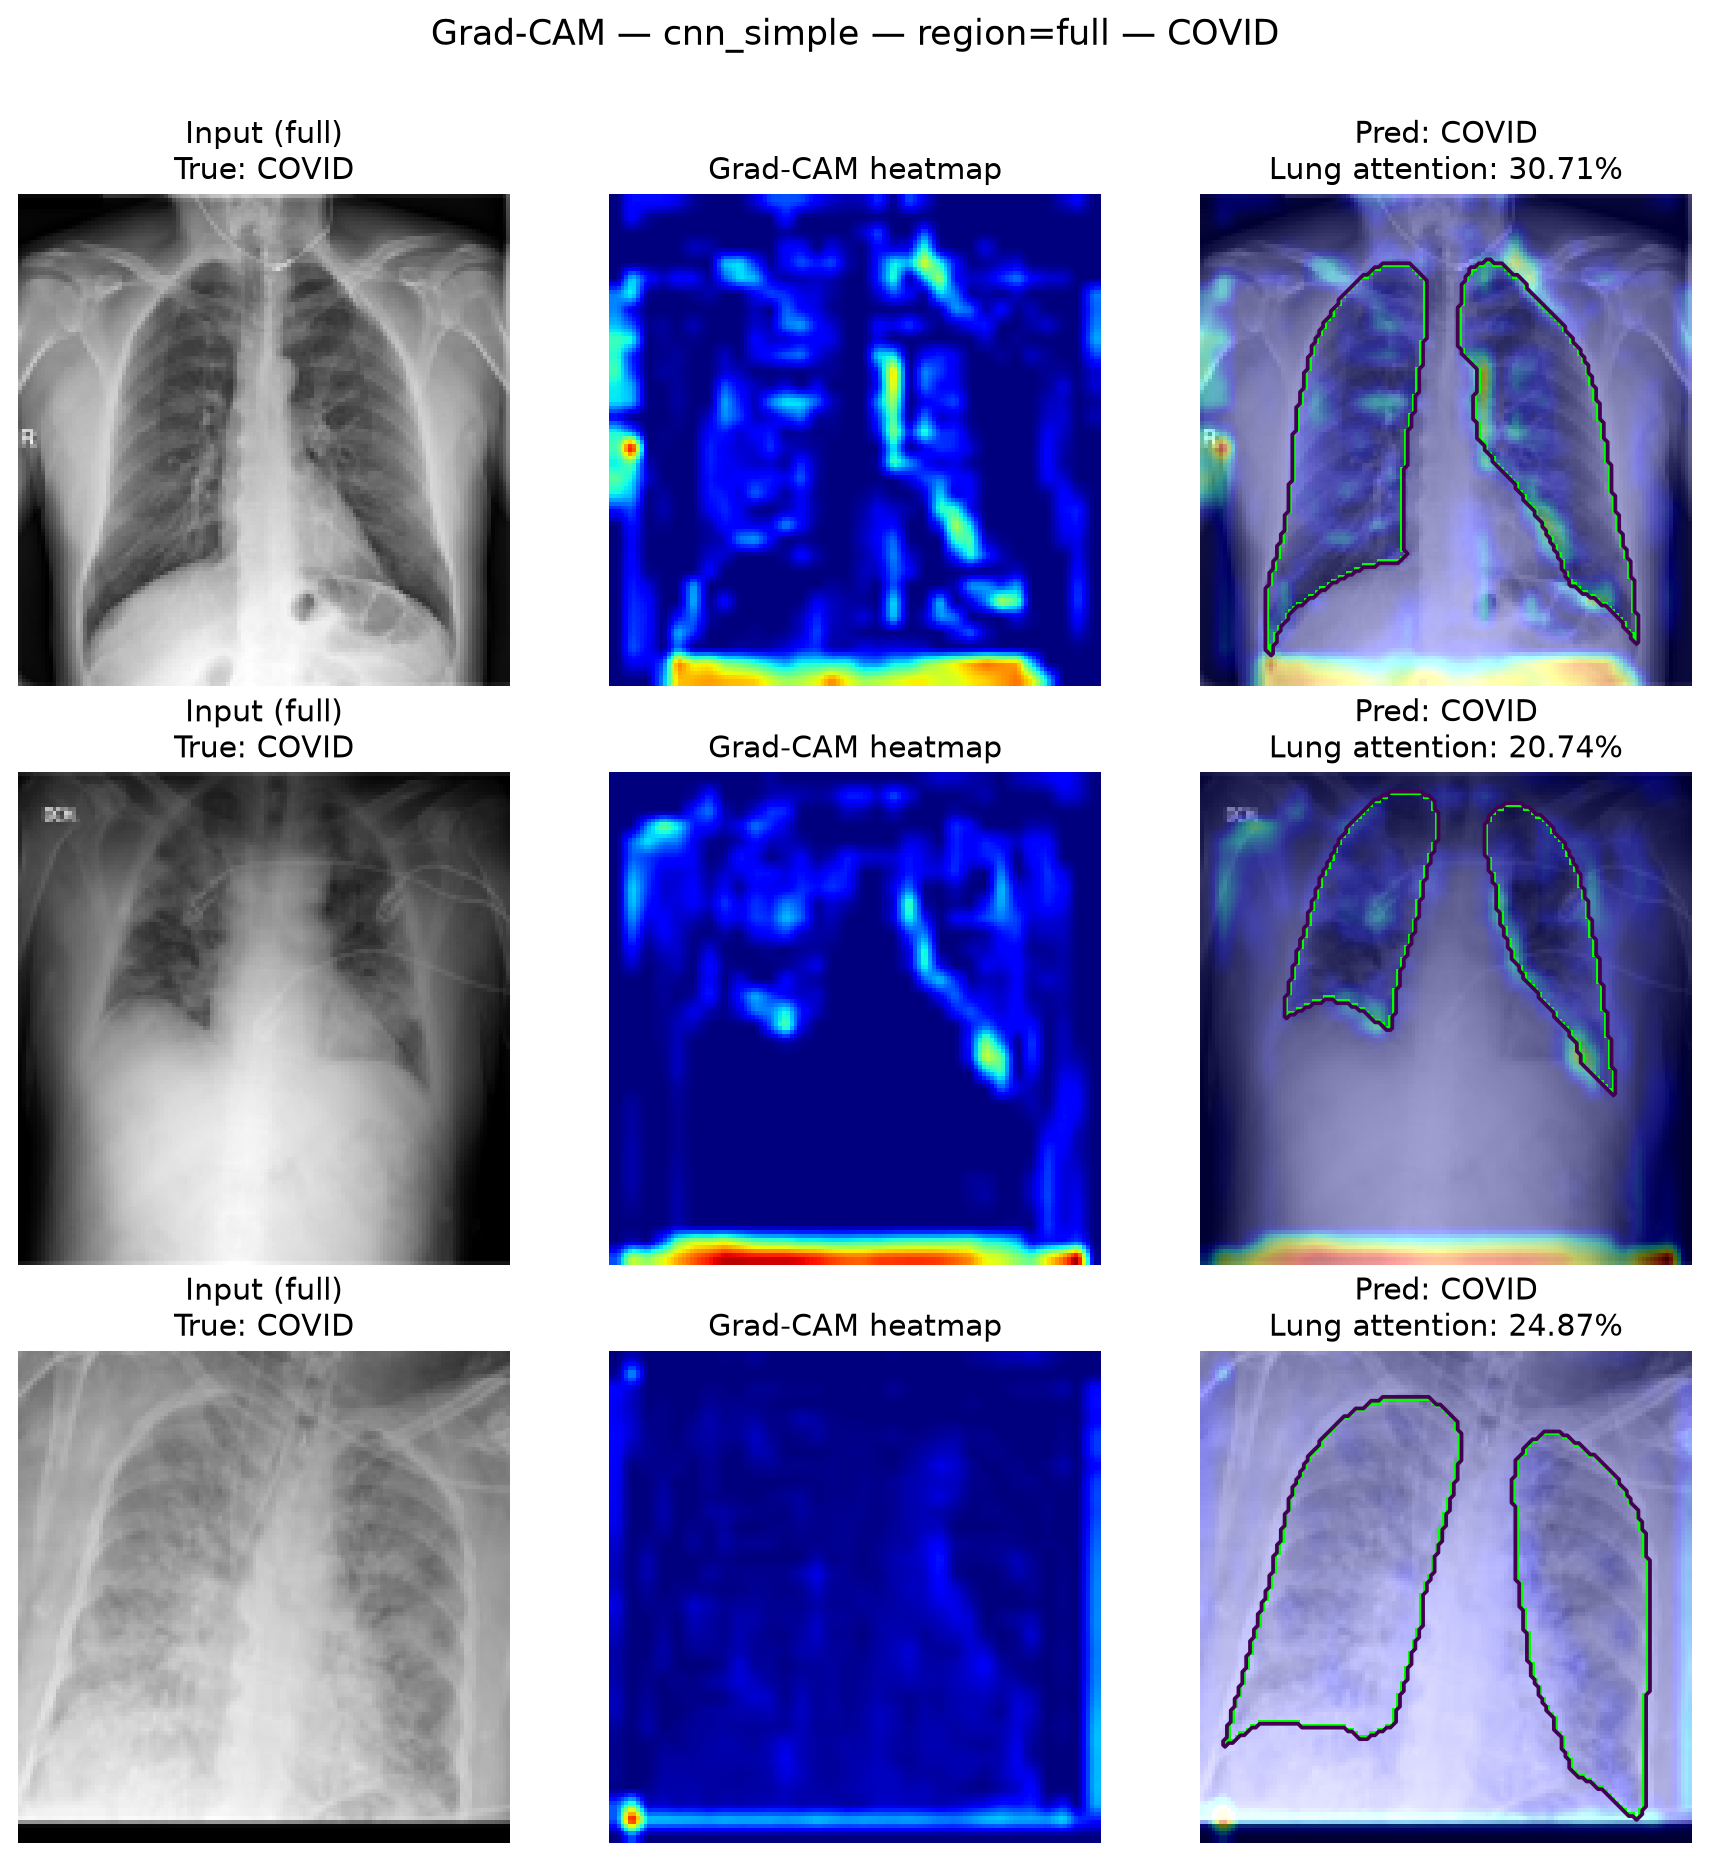
\includegraphics[width=\linewidth]{figures/gradcam_full_COVID.png}
        \caption{COVID}
    \end{subfigure}
    \hfill
    \begin{subfigure}{0.48\textwidth}
        \centering
        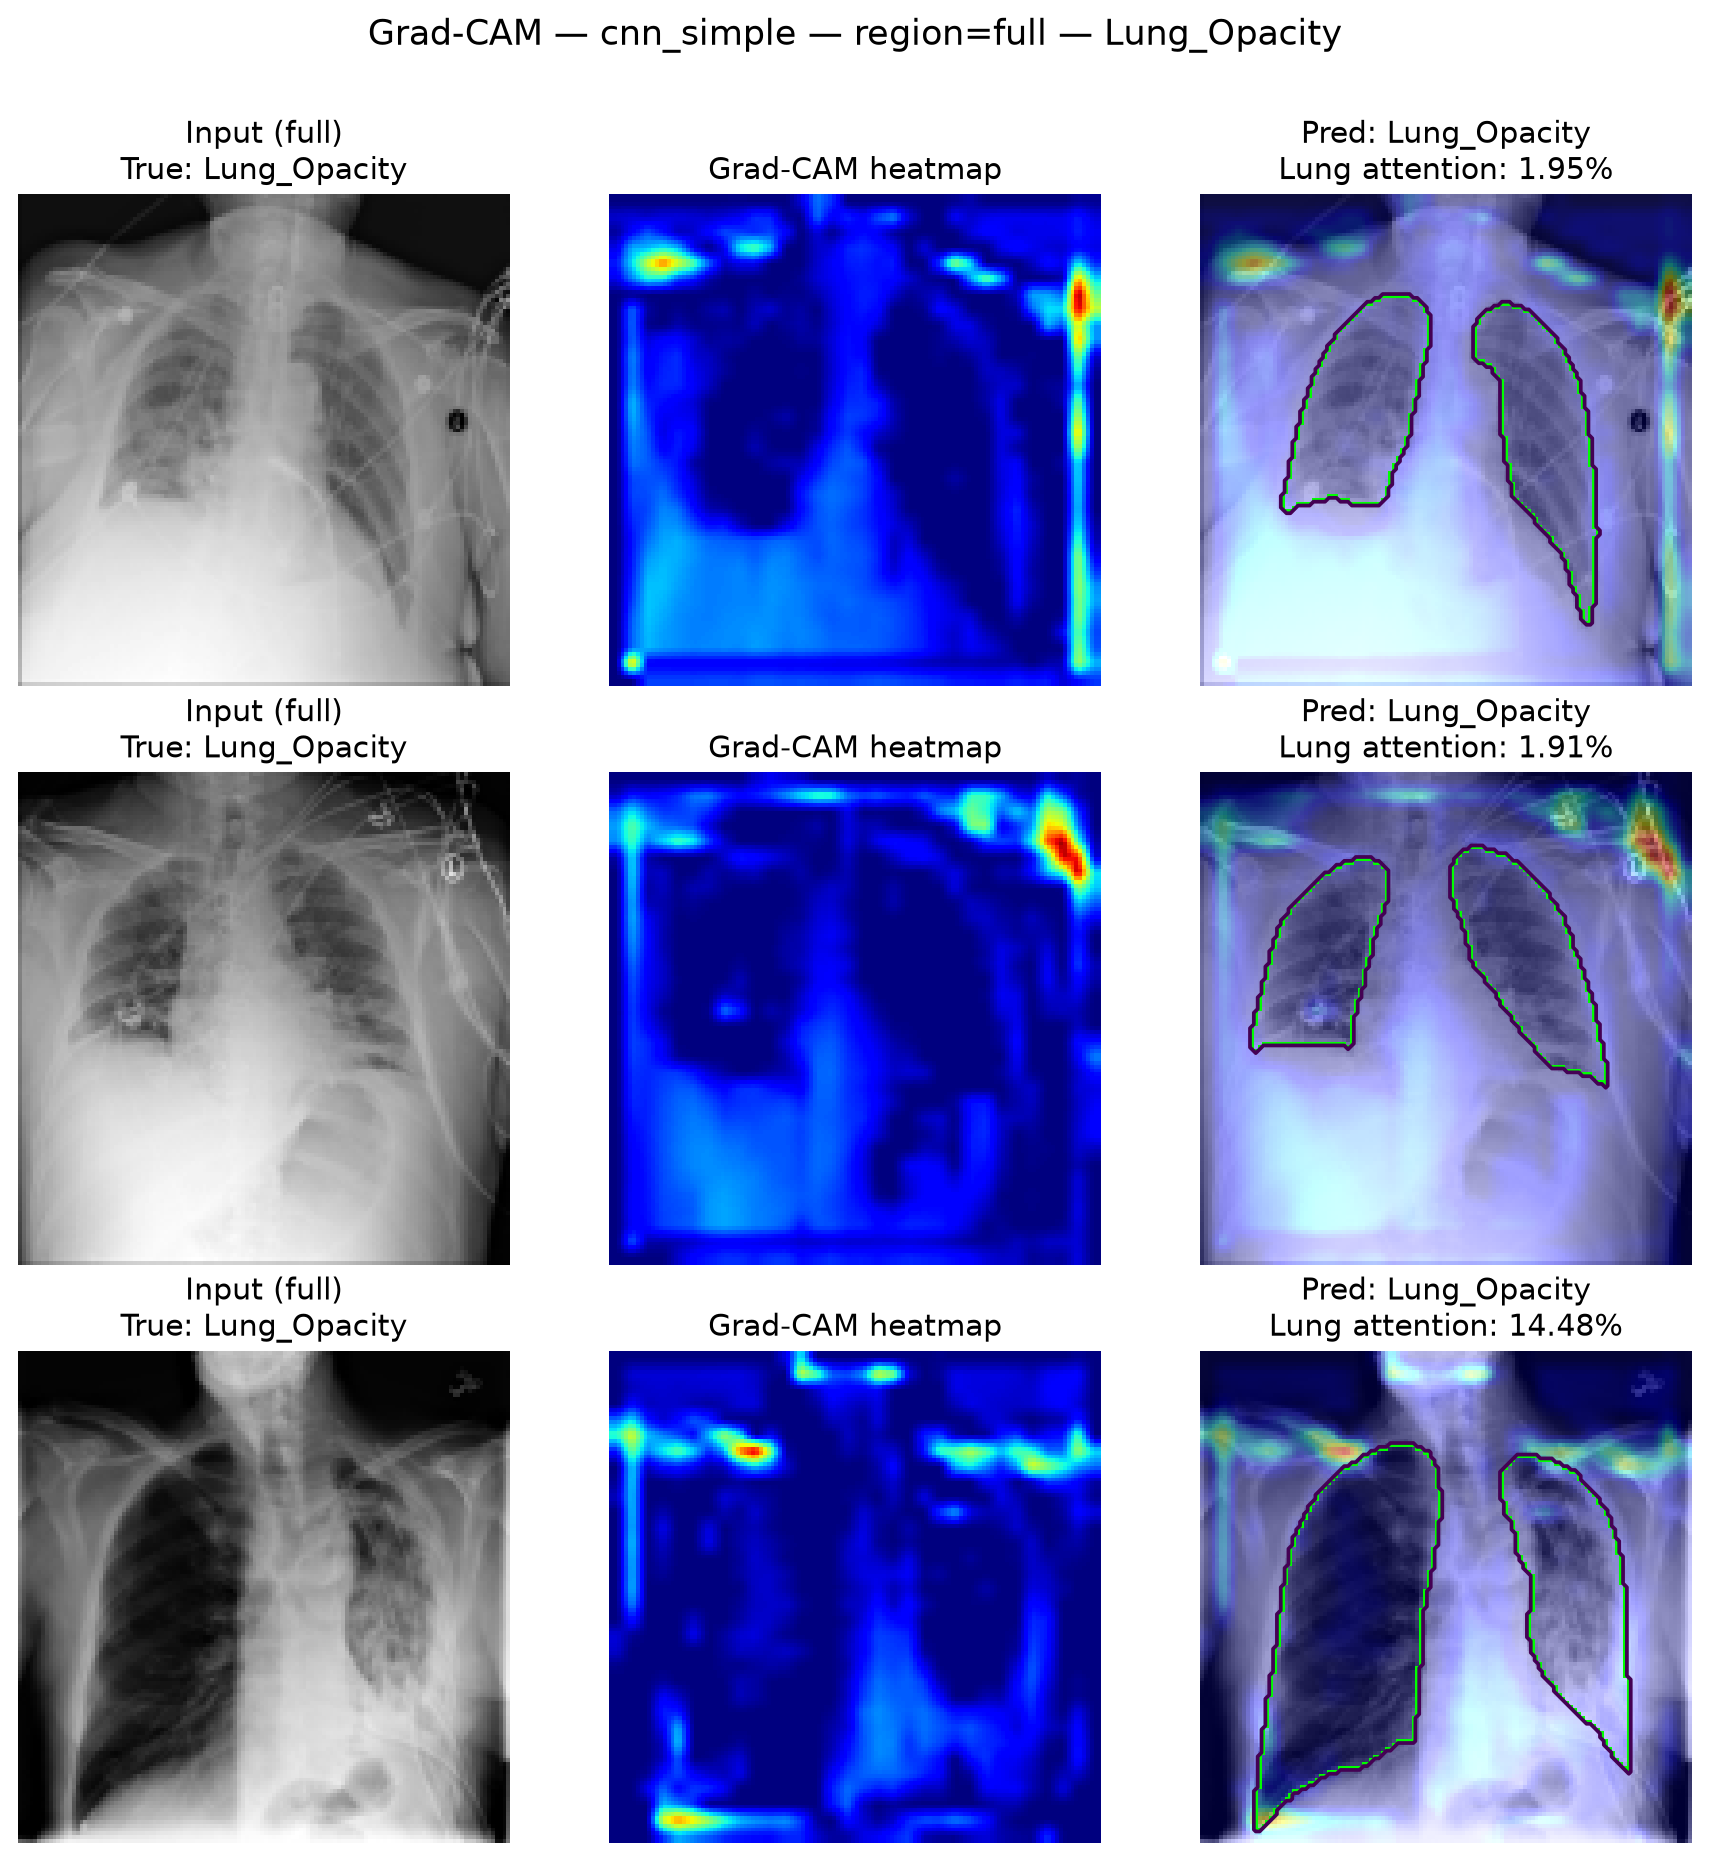
\includegraphics[width=\linewidth]{figures/gradcam_full_Lung_Opacity.png}
        \caption{Lung Opacity}
    \end{subfigure}

    \vspace{0.5em}

    \begin{subfigure}{0.48\textwidth}
        \centering
        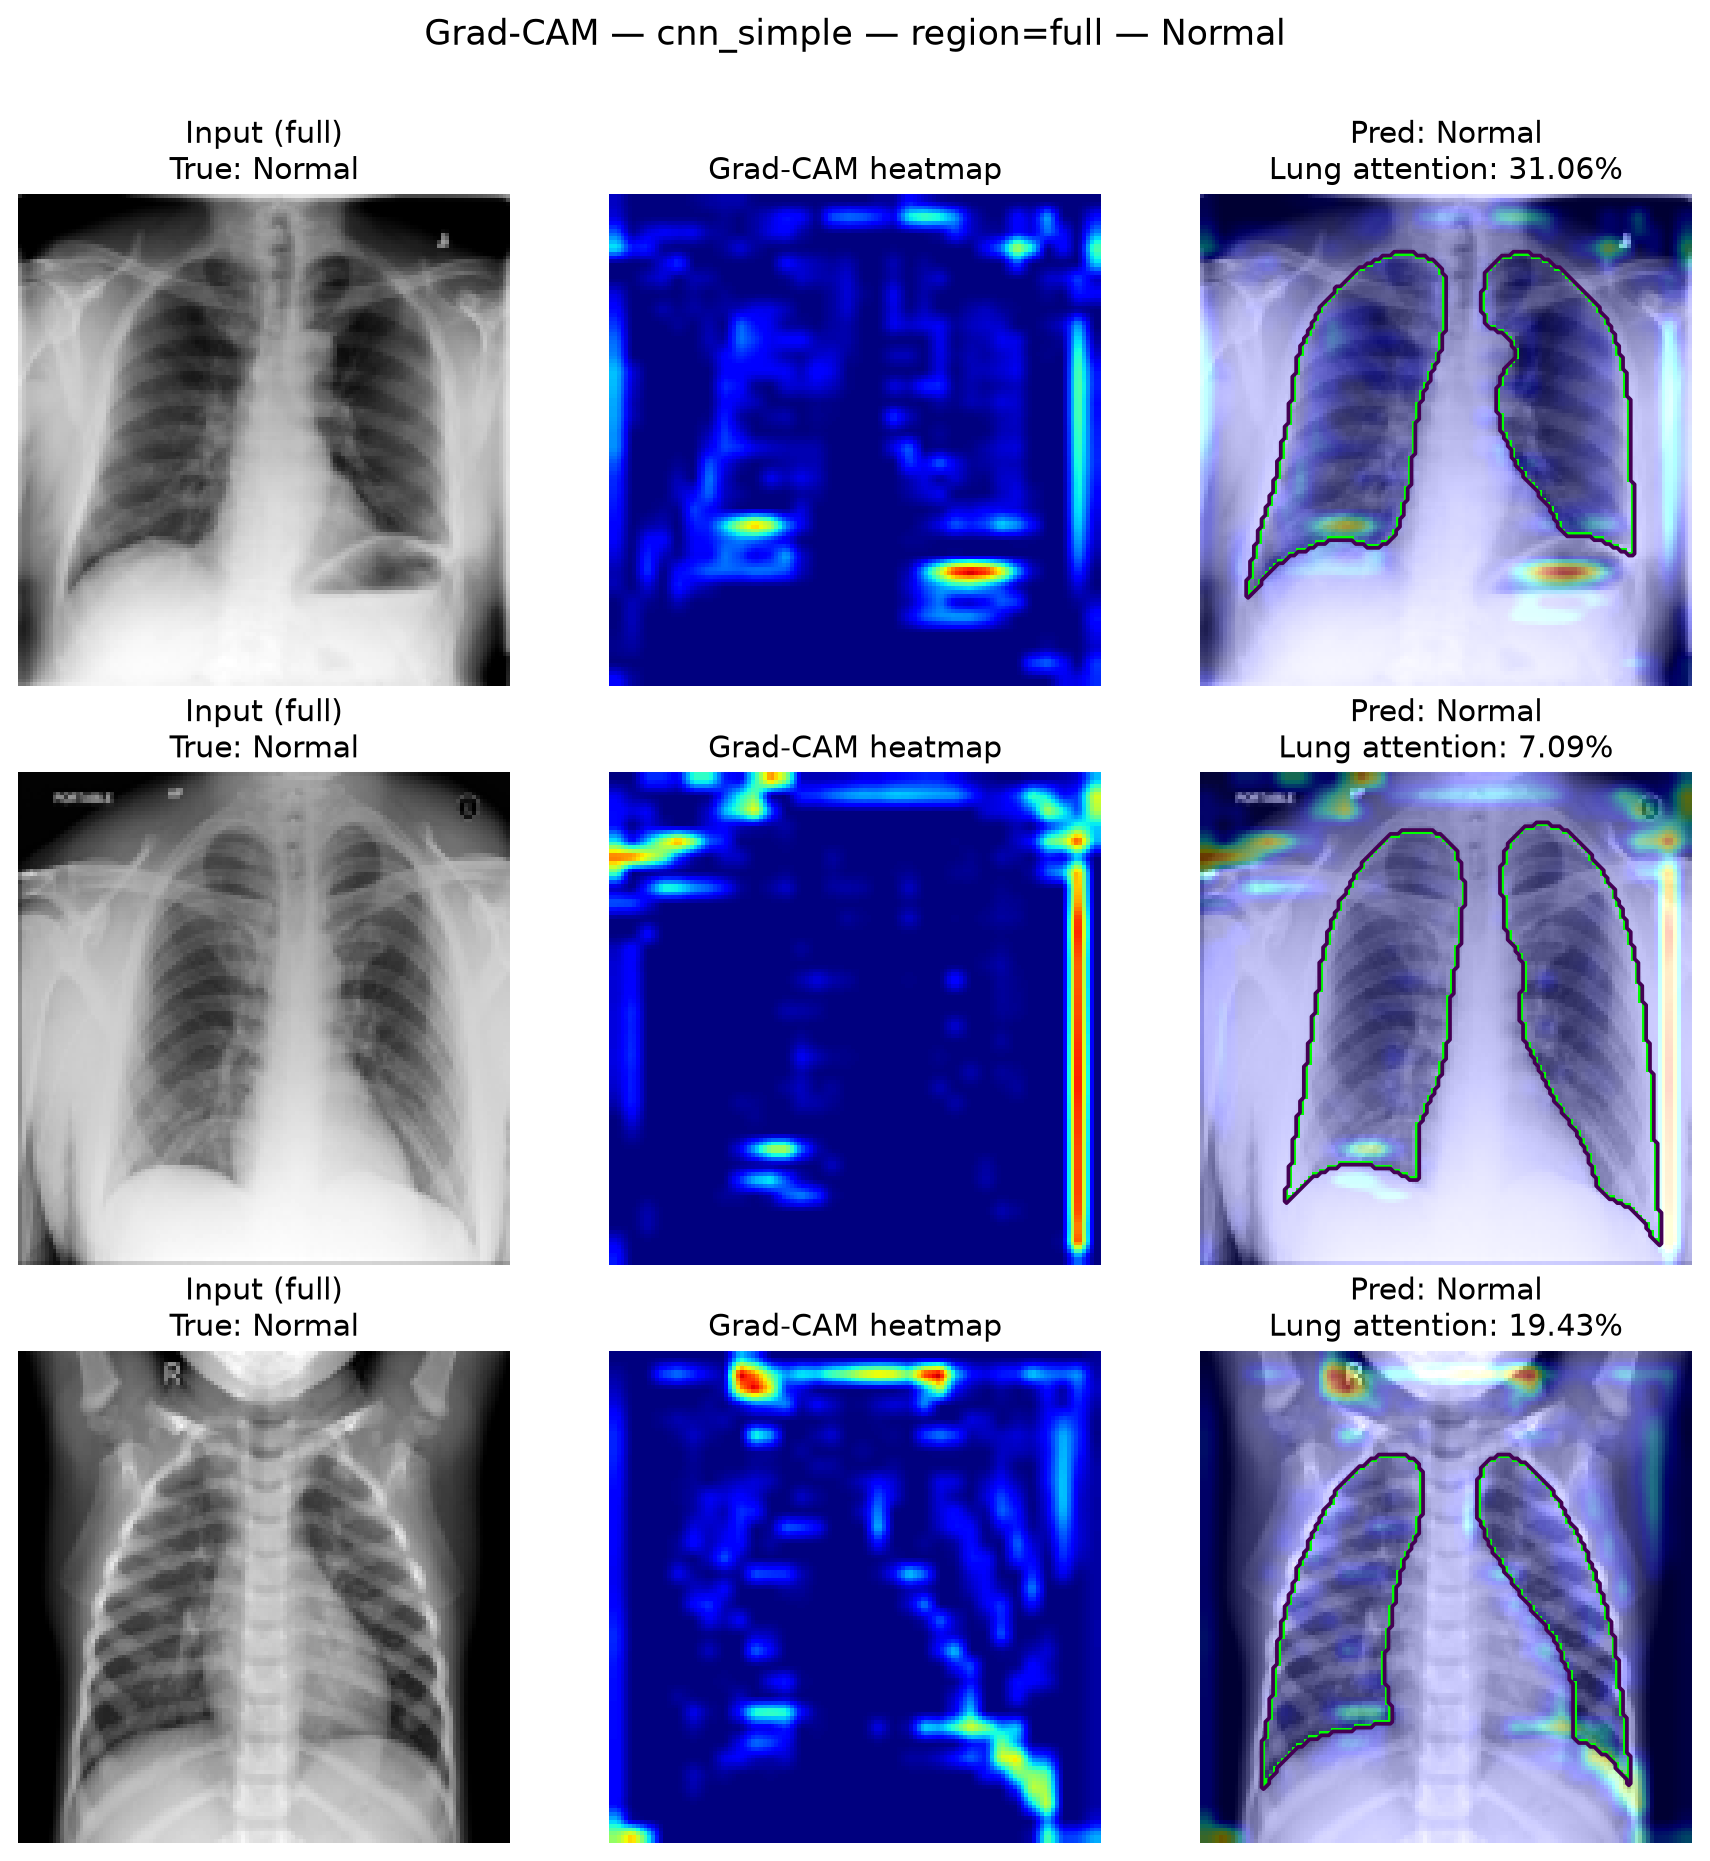
\includegraphics[width=\linewidth]{figures/gradcam_full_Normal.png}
        \caption{Normal}
    \end{subfigure}
    \hfill
    \begin{subfigure}{0.48\textwidth}
        \centering
        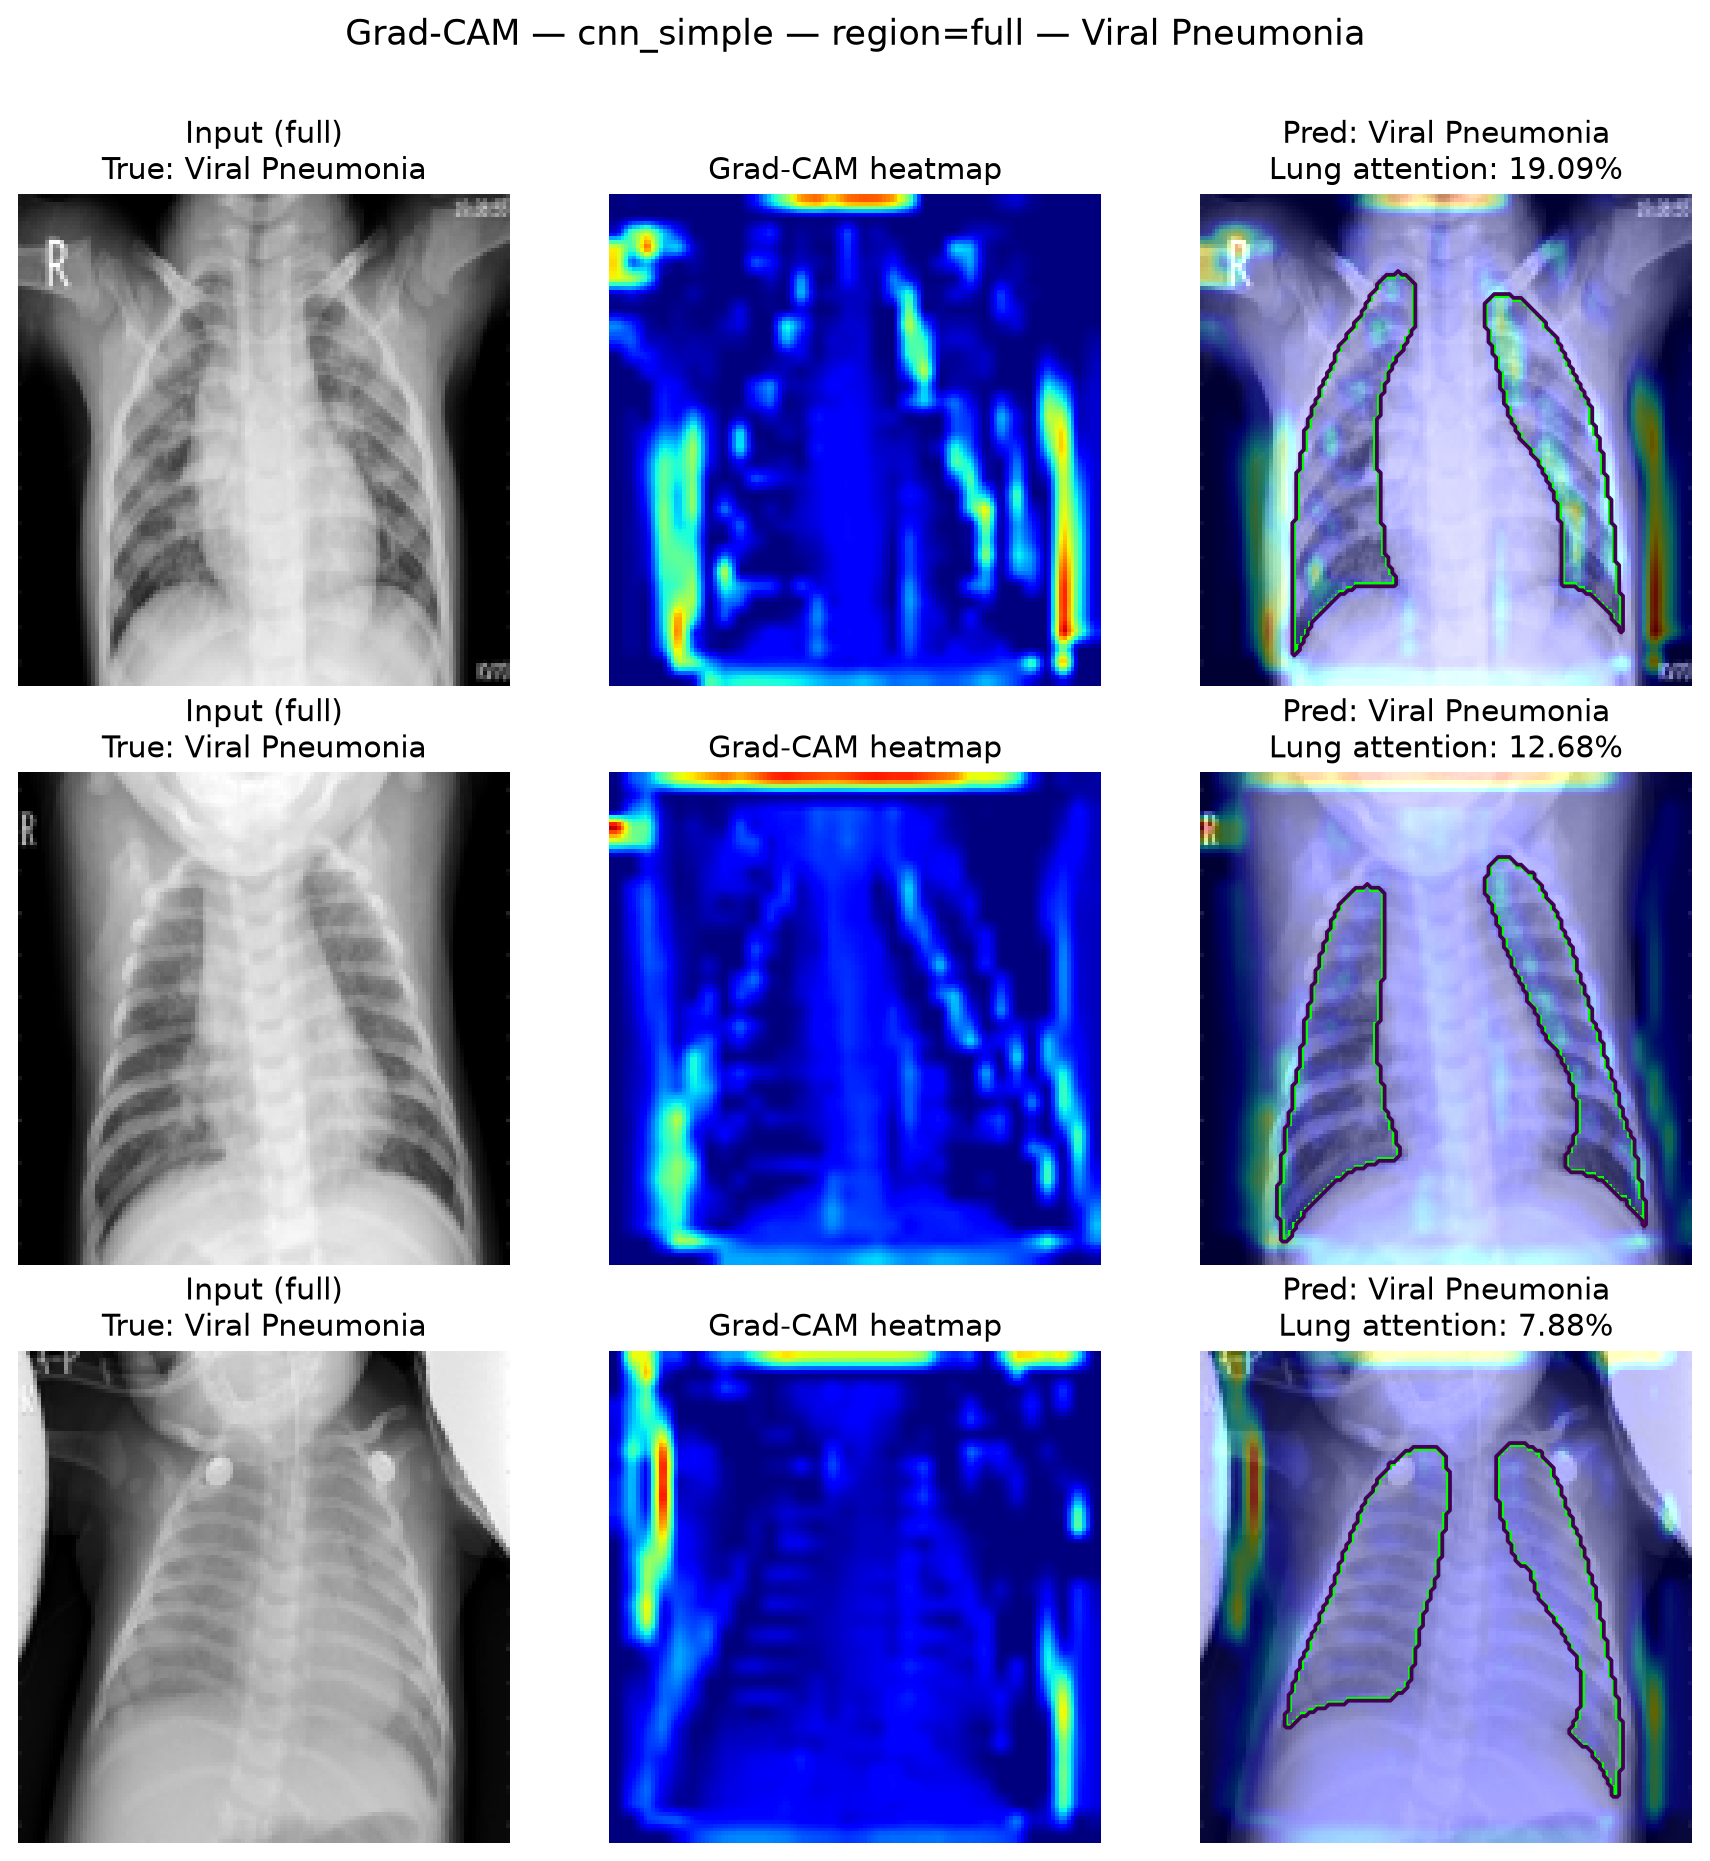
\includegraphics[width=\linewidth]{figures/gradcam_full_Viral_Pneumonia.png}
        \caption{Viral Pneumonia}
    \end{subfigure}

    \caption{Representative Grad-CAM examples for the full lung baseline, grouped by class.}
    \label{fig:gradcam_full}
\end{figure}

\subsection{Motivation for a Lung-Centred ROI Baseline}
\label{subsec:roi_motivation}

A hard lung-masking experiment was initially used to restrict the CNN to the
segmented pulmonary regions. This model achieved 72.93\% test accuracy and
69.0\% macro F1. However, hard masking introduced a sharp artificial boundary
between the retained lung pixels and the zero-valued background.

Grad-CAM visualisations frequently showed activation around these segmentation
boundaries. Consequently, the reduction in performance could not be attributed
solely to the removal of background information, because the masking operation
itself changed the image representation and potentially introduced new
geometric cues.

To obtain a cleaner controlled baseline, a lung-centred ROI preprocessing
strategy was therefore introduced.

\subsection{Baseline 2: Lung-ROI Simple CNN}
\label{subsec:roi_baseline}

For the second baseline, lung segmentation masks were used only to determine
the spatial extent of the lungs. The image itself was not multiplied by the
mask.

The preprocessing pipeline was:

\begin{enumerate}
    \item Load the original chest X-ray and corresponding lung mask.
    \item Use the mask to determine the joint bounding box of the two lungs.
    \item Add a small spatial margin around the lung region.
    \item Construct a square ROI around the lung pair.
    \item Preserve the original radiographic intensities and anatomical
    appearance.
    \item Resize the ROI to $128 \times 128$ pixels.
\end{enumerate}

This preprocessing reduced variation in overall framing and lung scale while
avoiding hard segmentation boundaries. No rotation normalisation, intensity
normalisation, or augmentation was applied.

\begin{figure}[H]
    \centering

    \begin{subfigure}{0.48\textwidth}
        \centering
        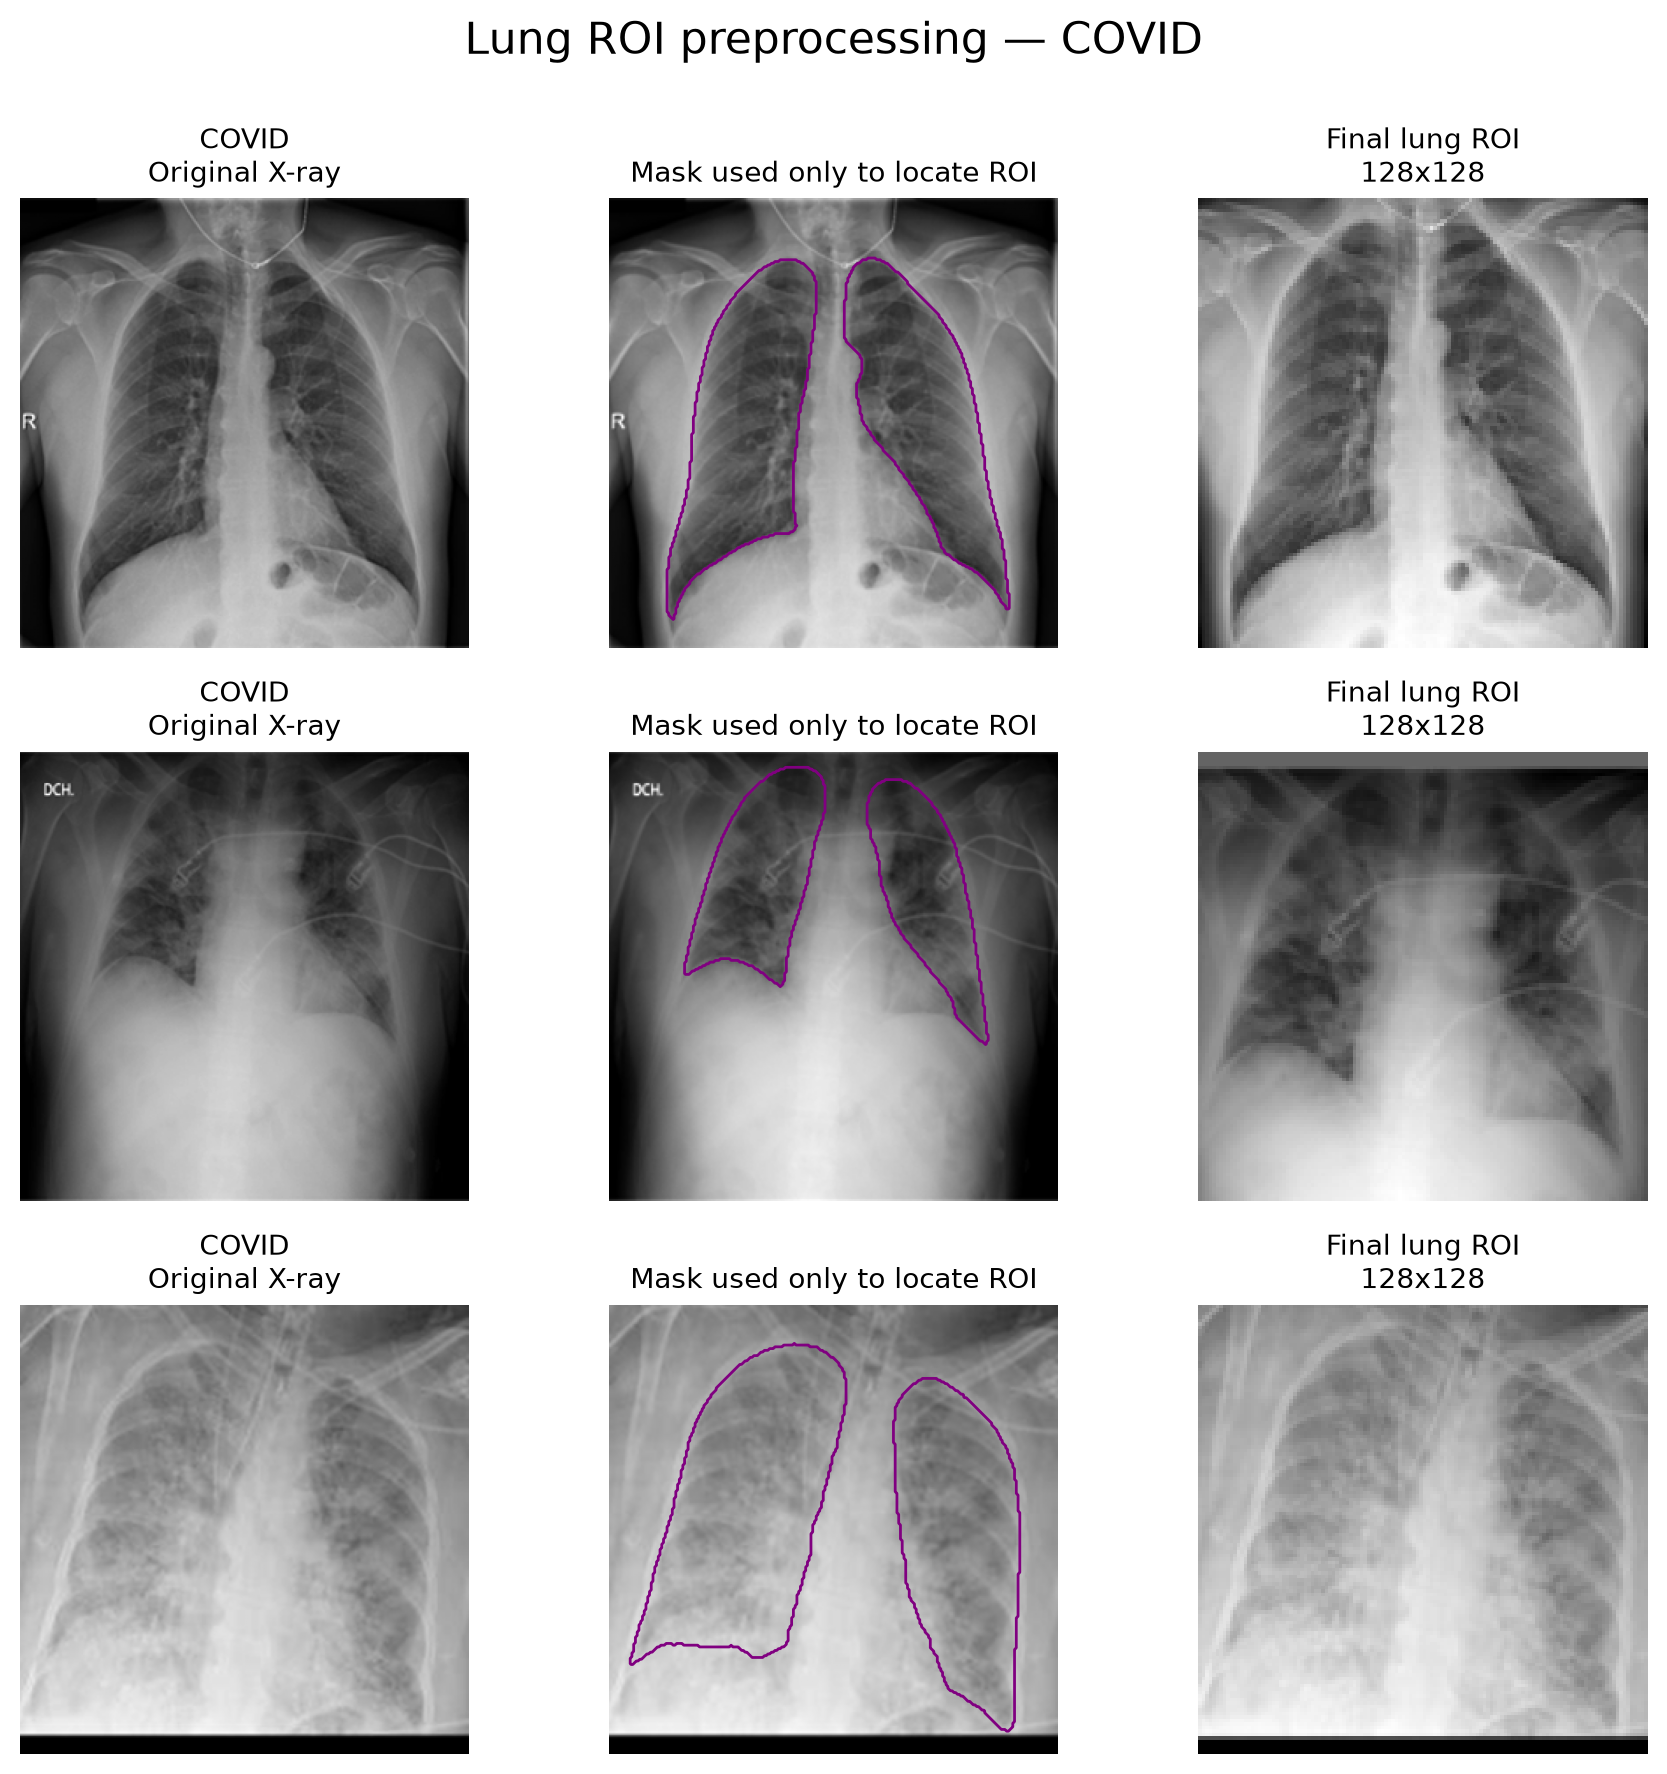
\includegraphics[width=\linewidth]{figures/lung_roi_covid.png}
        \caption{COVID}
    \end{subfigure}
    \hfill
    \begin{subfigure}{0.48\textwidth}
        \centering
        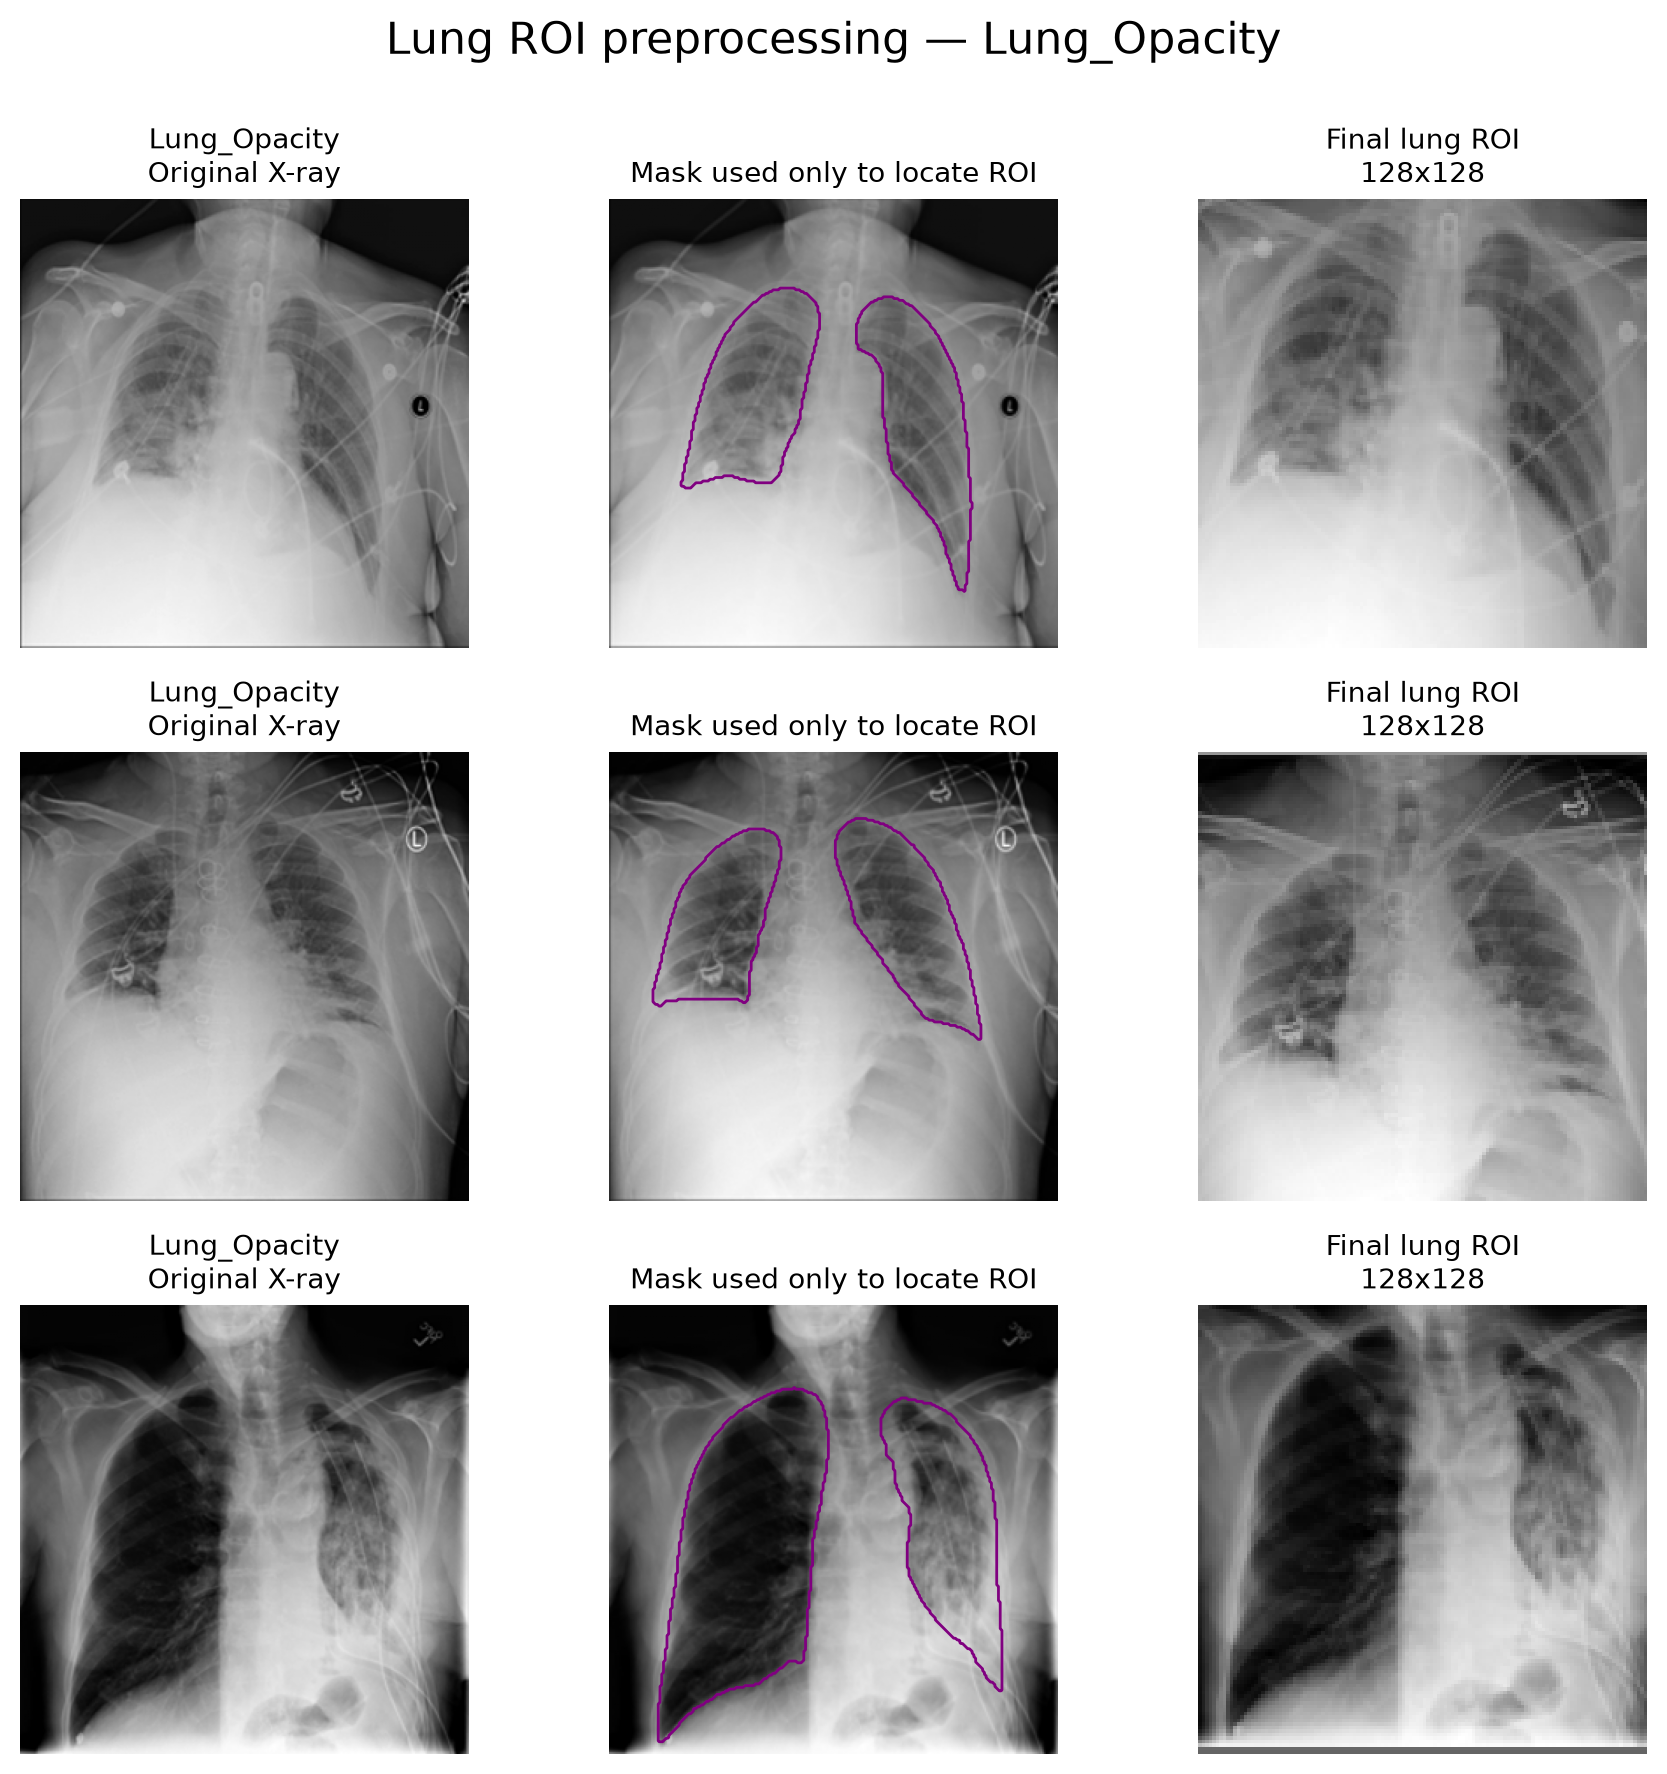
\includegraphics[width=\linewidth]{figures/lung_roi_lung_opacity.png}
        \caption{Lung Opacity}
    \end{subfigure}

    \vspace{0.5em}

    \begin{subfigure}{0.48\textwidth}
        \centering
        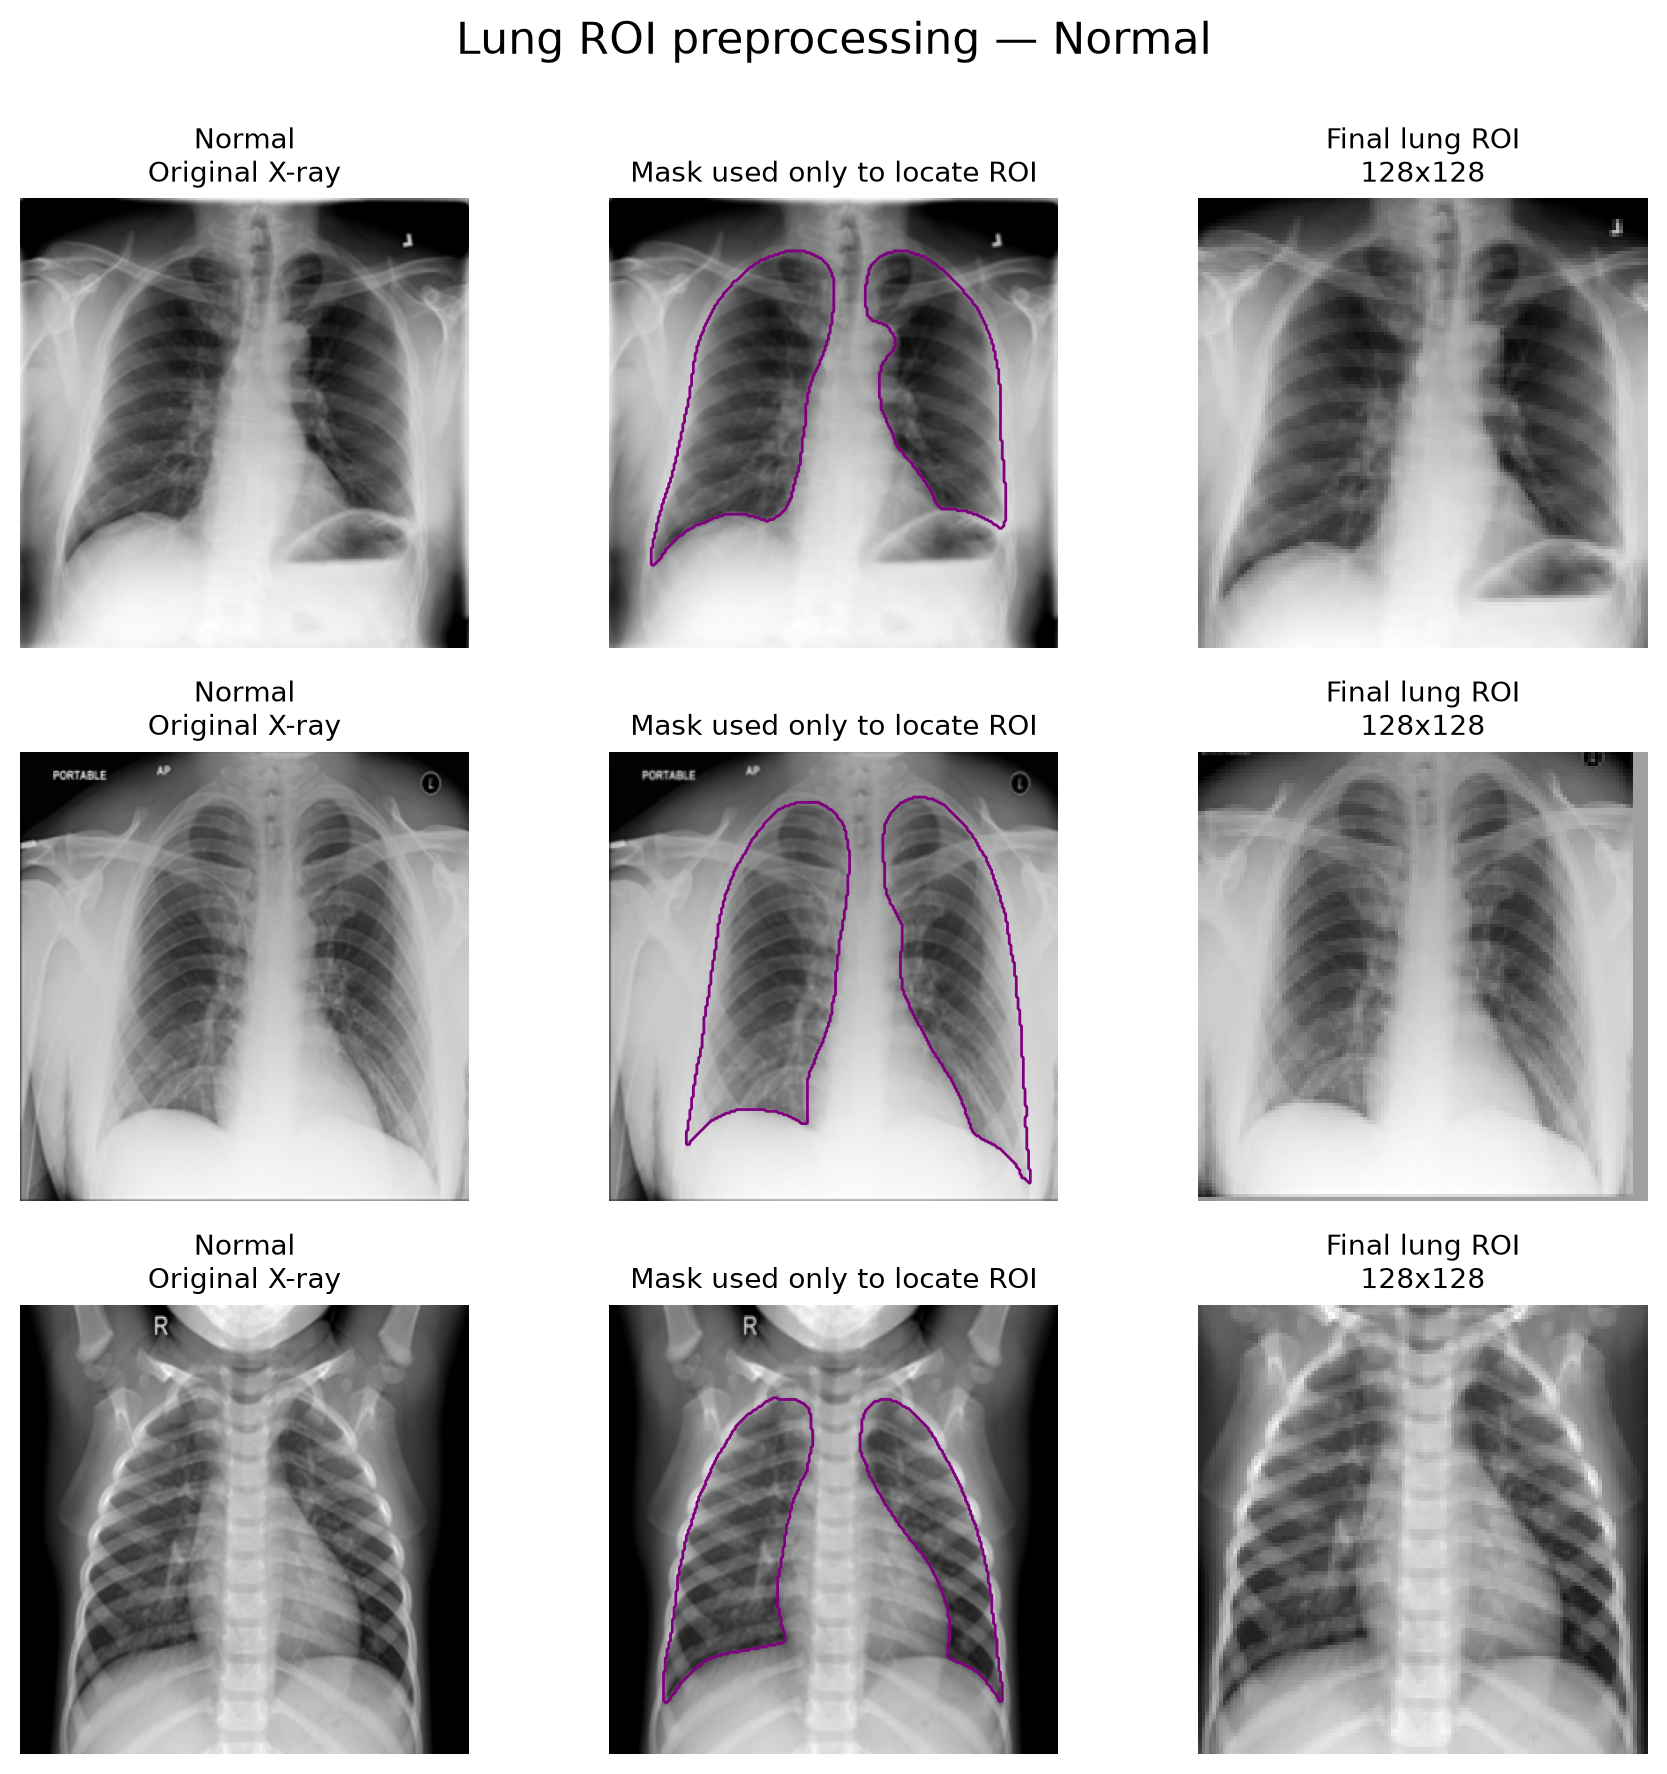
\includegraphics[width=\linewidth]{figures/lung_roi_normal.png}
        \caption{Normal}
    \end{subfigure}
    \hfill
    \begin{subfigure}{0.48\textwidth}
        \centering
        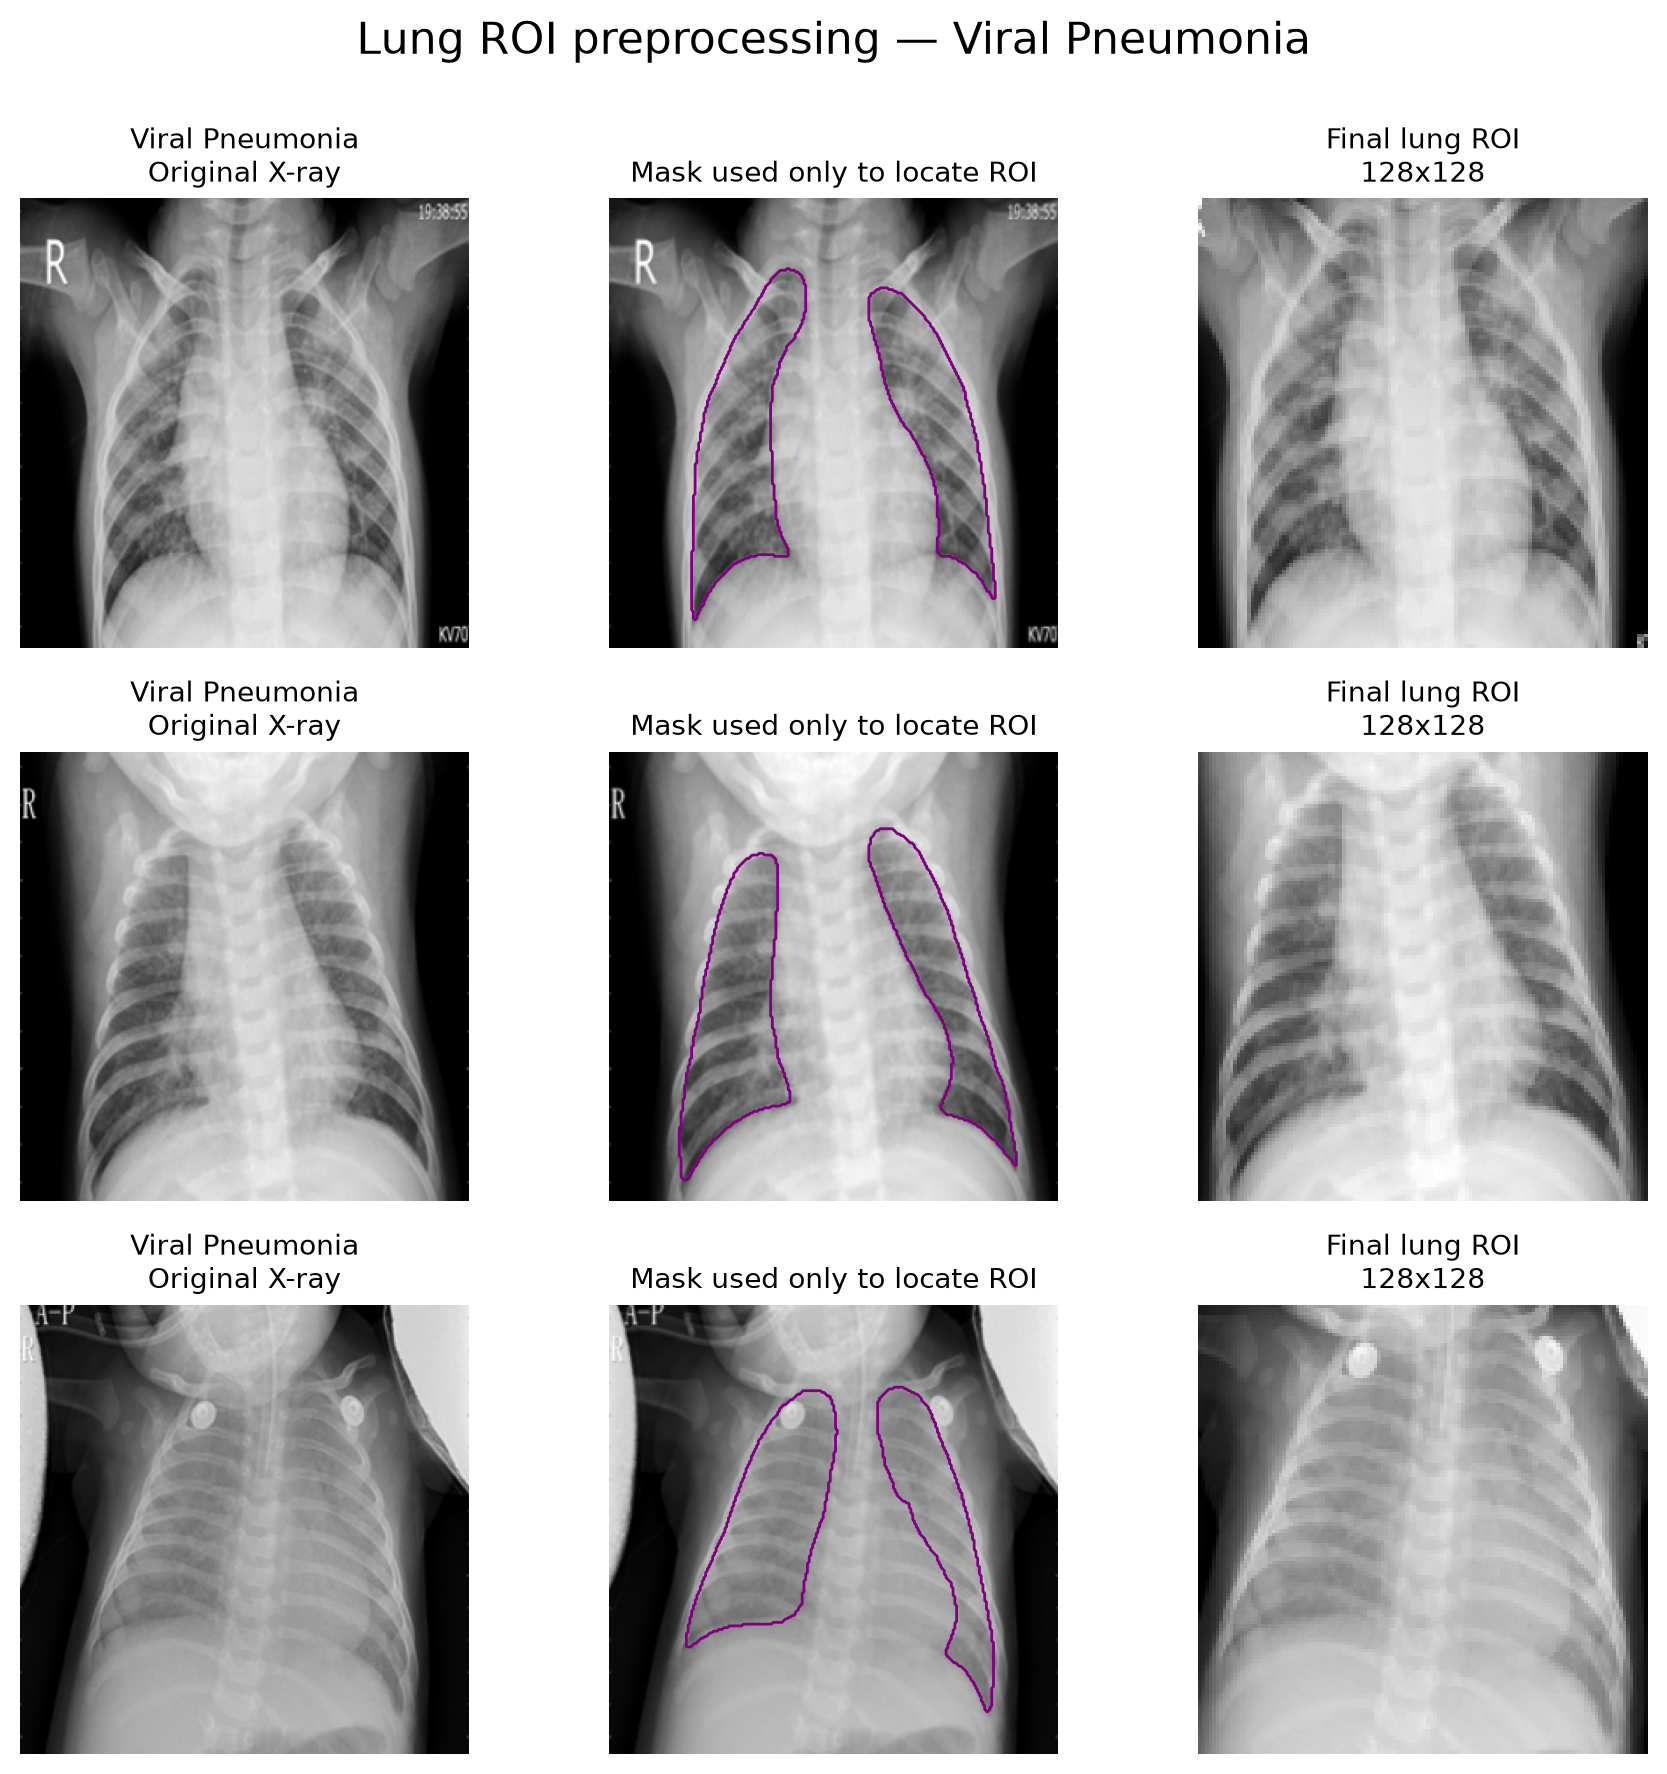
\includegraphics[width=\linewidth]{figures/lung_roi_viral_pneumonia.png}
        \caption{Viral Pneumonia}
    \end{subfigure}

    \caption{
        Class-wise examples of the lung-centred ROI preprocessing pipeline.
    }
    \label{fig:lung-roi-preprocessing-by-class}
\end{figure}

The lung-ROI model achieved the test-set performance shown in
Table~\ref{tab:roi_baseline_results}.

\begin{table}[H]
\centering
\caption{Test-set performance of the lung-ROI simple CNN baseline.}
\label{tab:roi_baseline_results}
\begin{tabular}{lccc}
\toprule
\textbf{Class} & \textbf{Precision} & \textbf{Recall} & \textbf{F1-score} \\
\midrule
COVID            & 0.649 & 0.703 & 0.675 \\
Lung Opacity     & 0.822 & 0.691 & 0.751 \\
Normal           & 0.828 & 0.853 & 0.840 \\
Viral Pneumonia  & 0.746 & 0.940 & 0.832 \\
\midrule
\textbf{Macro average} & 0.761 & 0.797 & \textbf{0.774} \\
\bottomrule
\end{tabular}
\end{table}

The lung-ROI model achieved \textbf{78.71\% test accuracy} and
\textbf{77.4\% macro F1}. Its train, validation, and test accuracies were
79.86\%, 78.74\%, and 78.71\%, respectively, indicating close agreement between
the data partitions and little evidence of severe overfitting.

\subsection{Comparison of the Two Baselines}
\label{subsec:baseline_comparison}

Table~\ref{tab:baseline_comparison} compares the two principal baselines.

\begin{table}[H]
\centering
\caption{Comparison of the two principal simple-CNN baselines.}
\label{tab:baseline_comparison}
\begin{tabular}{lcc}
\toprule
\textbf{Baseline} & \textbf{Test Accuracy} & \textbf{Macro F1} \\
\midrule
Full-image simple CNN & \textbf{81.96\%} & \textbf{82.7\%} \\
Lung-ROI simple CNN   & 78.71\% & 77.4\% \\
\bottomrule
\end{tabular}
\end{table}

Restricting the model to the lung-centred ROI reduced test accuracy by
3.25 percentage points and macro F1 by 5.3 percentage points. Nevertheless,
the ROI model retained a substantial proportion of the full-image
classification performance.

The class-wise recall comparison is shown in
Table~\ref{tab:baseline_recall_comparison}.

\begin{table}[H]
\centering
\caption{Class-wise recall of the full-image and lung-ROI baselines.}
\label{tab:baseline_recall_comparison}
\begin{tabular}{lcc}
\toprule
\textbf{Class} & \textbf{Full Image} & \textbf{Lung ROI} \\
\midrule
COVID            & \textbf{83.0\%} & 70.3\% \\
Lung Opacity     & \textbf{76.6\%} & 69.1\% \\
Normal           & 83.1\% & \textbf{85.3\%} \\
Viral Pneumonia  & \textbf{94.5\%} & 94.0\% \\
\bottomrule
\end{tabular}
\end{table}

The largest reduction occurred for COVID classification. In contrast, Normal
and Viral Pneumonia recall remained relatively stable.

These results suggest that peripheral image regions contribute to the
performance of the full-image model, but they are not the sole source of
discriminative information. A substantial level of classification performance
remained when the input was restricted to a lung-centred thoracic ROI.

\subsection{Grad-CAM Analysis of the Lung-ROI Baseline}
\label{subsec:roi_gradcam}

Grad-CAM was also applied to the lung-ROI baseline. Unlike the hard-masked
experiment, no artificial segmentation contour was present in the CNN input.
Therefore, activation outside the segmented lung contour corresponds to actual
anatomical or image regions contained within the ROI.

Qualitative inspection showed heterogeneous attention across the four classes.
COVID examples generally demonstrated a greater degree of pulmonary
activation, although attention was not exclusively confined to the lung
fields. In several Lung Opacity and Viral Pneumonia examples, correctly
classified images exhibited strong activation in peripheral, inferior,
mediastinal, or ROI-border regions despite relatively low activation within
the segmented pulmonary interior. Normal cases showed mixed behaviour, with both pulmonary and peripheral
activation patterns.

These observations suggest that ROI cropping substantially reduces peripheral
image information but does not completely prevent the CNN from exploiting
extra-pulmonary or framing-related cues within the cropped thoracic region.

Because this ROI Grad-CAM assessment is currently based on representative
qualitative examples rather than complete test-set quantitative attention
analysis, the findings are interpreted as exploratory.

\begin{figure}[H]
    \centering

    \begin{subfigure}{0.48\textwidth}
        \centering
        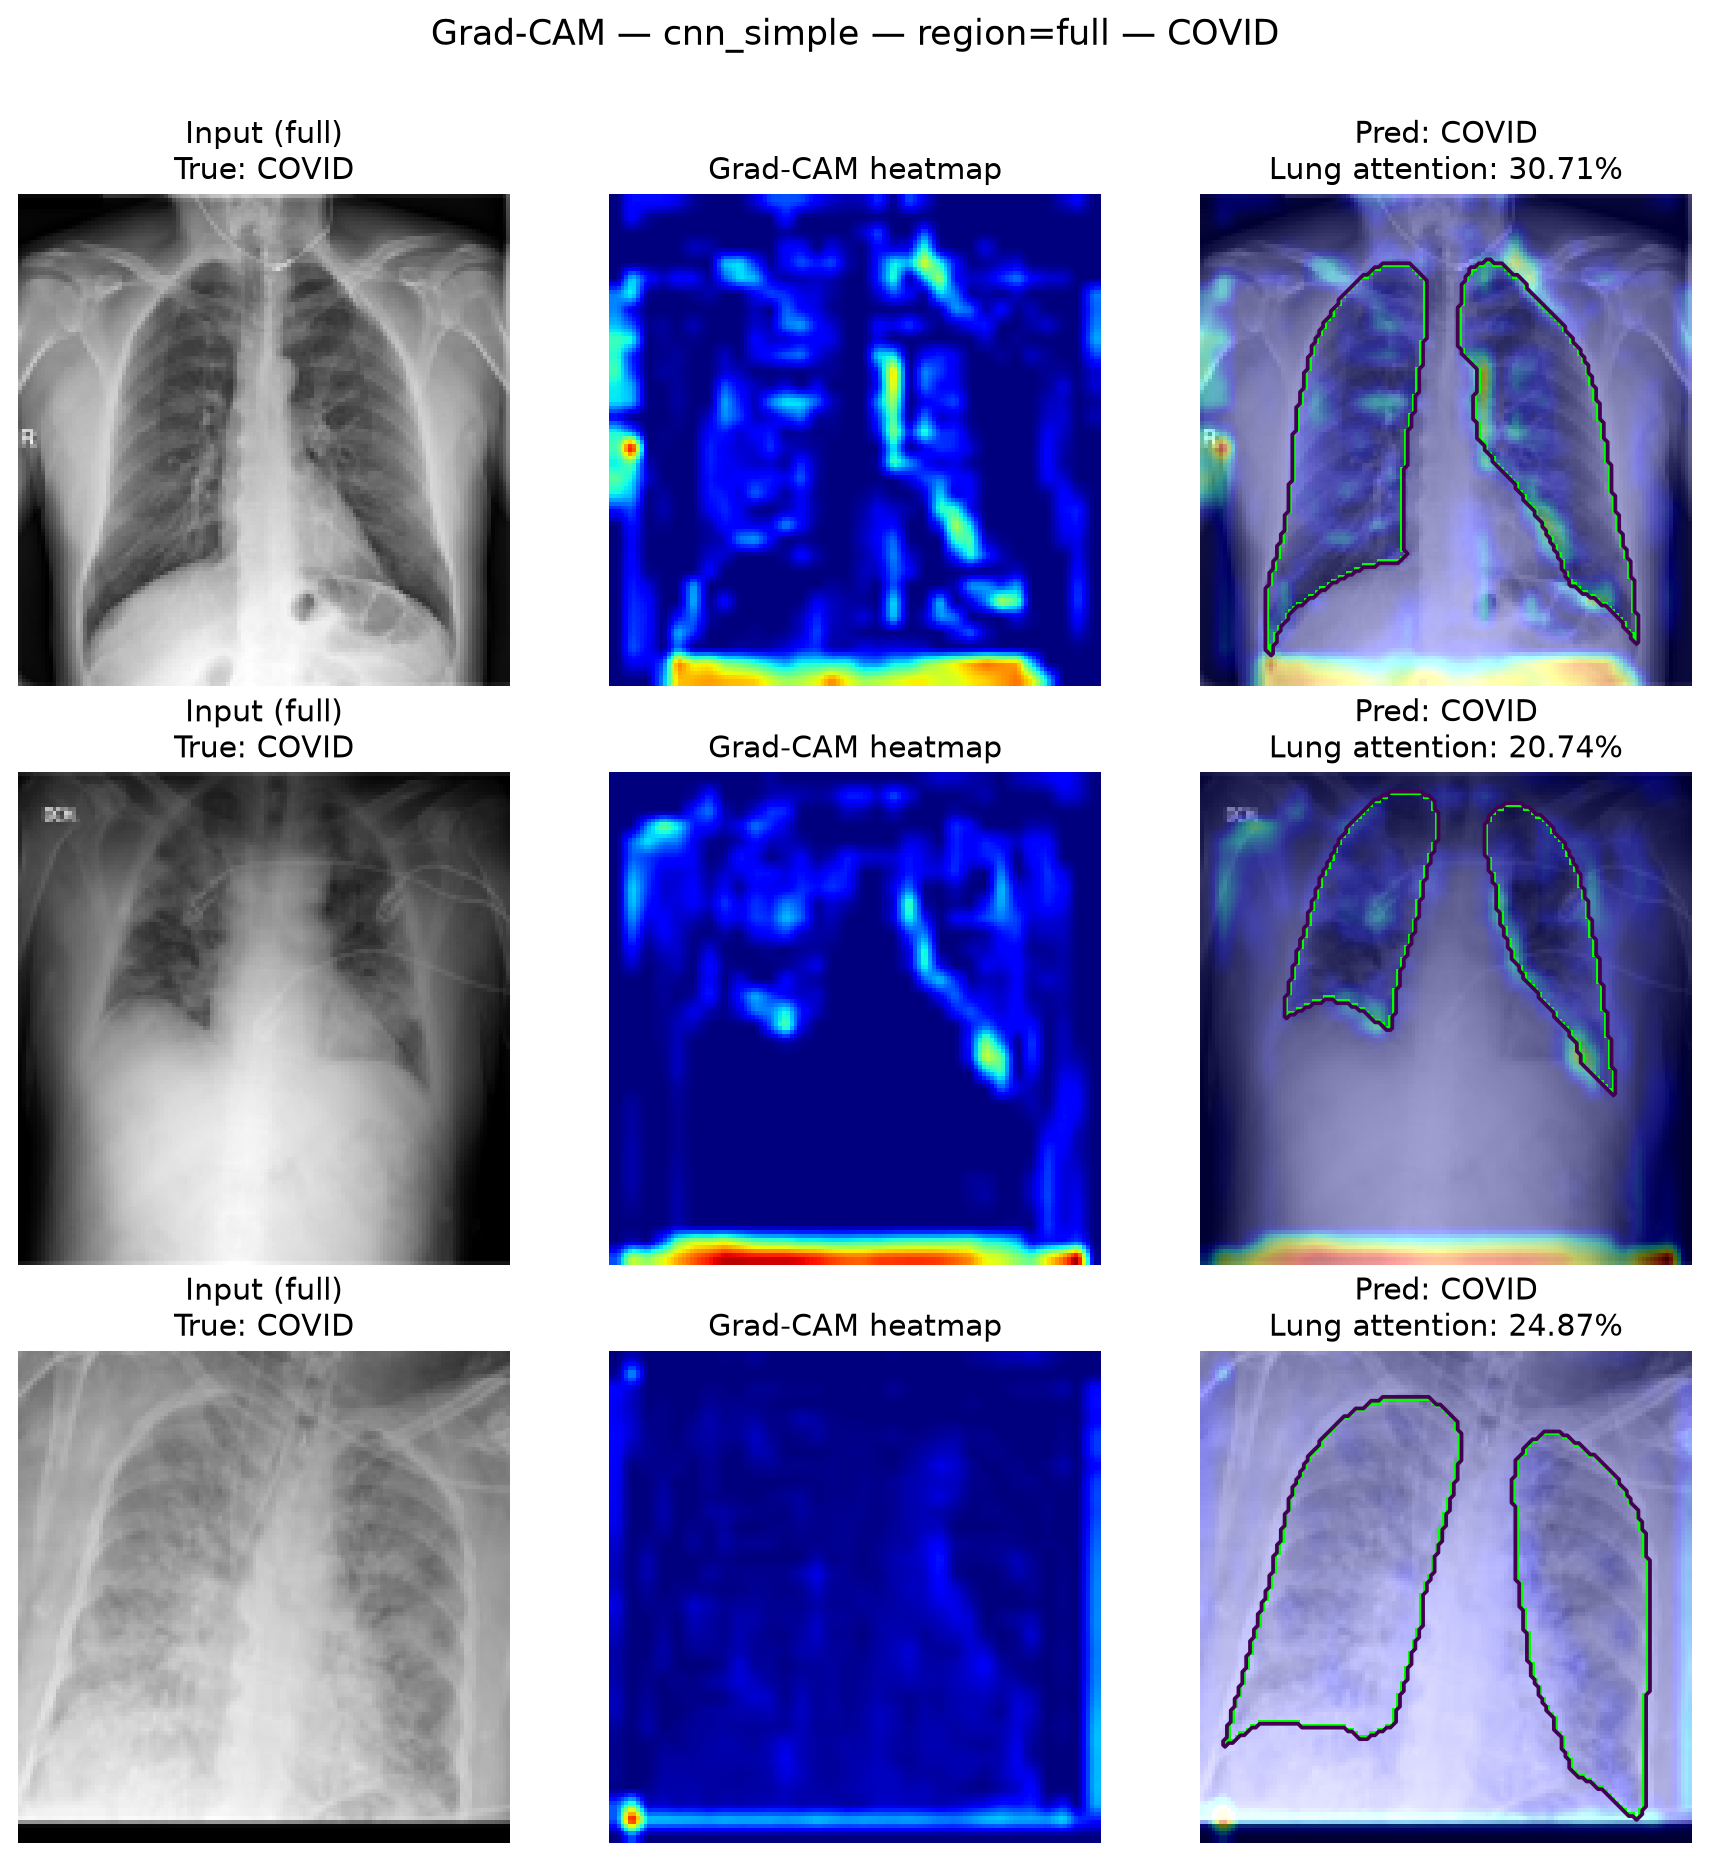
\includegraphics[width=\linewidth]{figures/gradcam_full_COVID.png}
        \caption{COVID}
    \end{subfigure}
    \hfill
    \begin{subfigure}{0.48\textwidth}
        \centering
        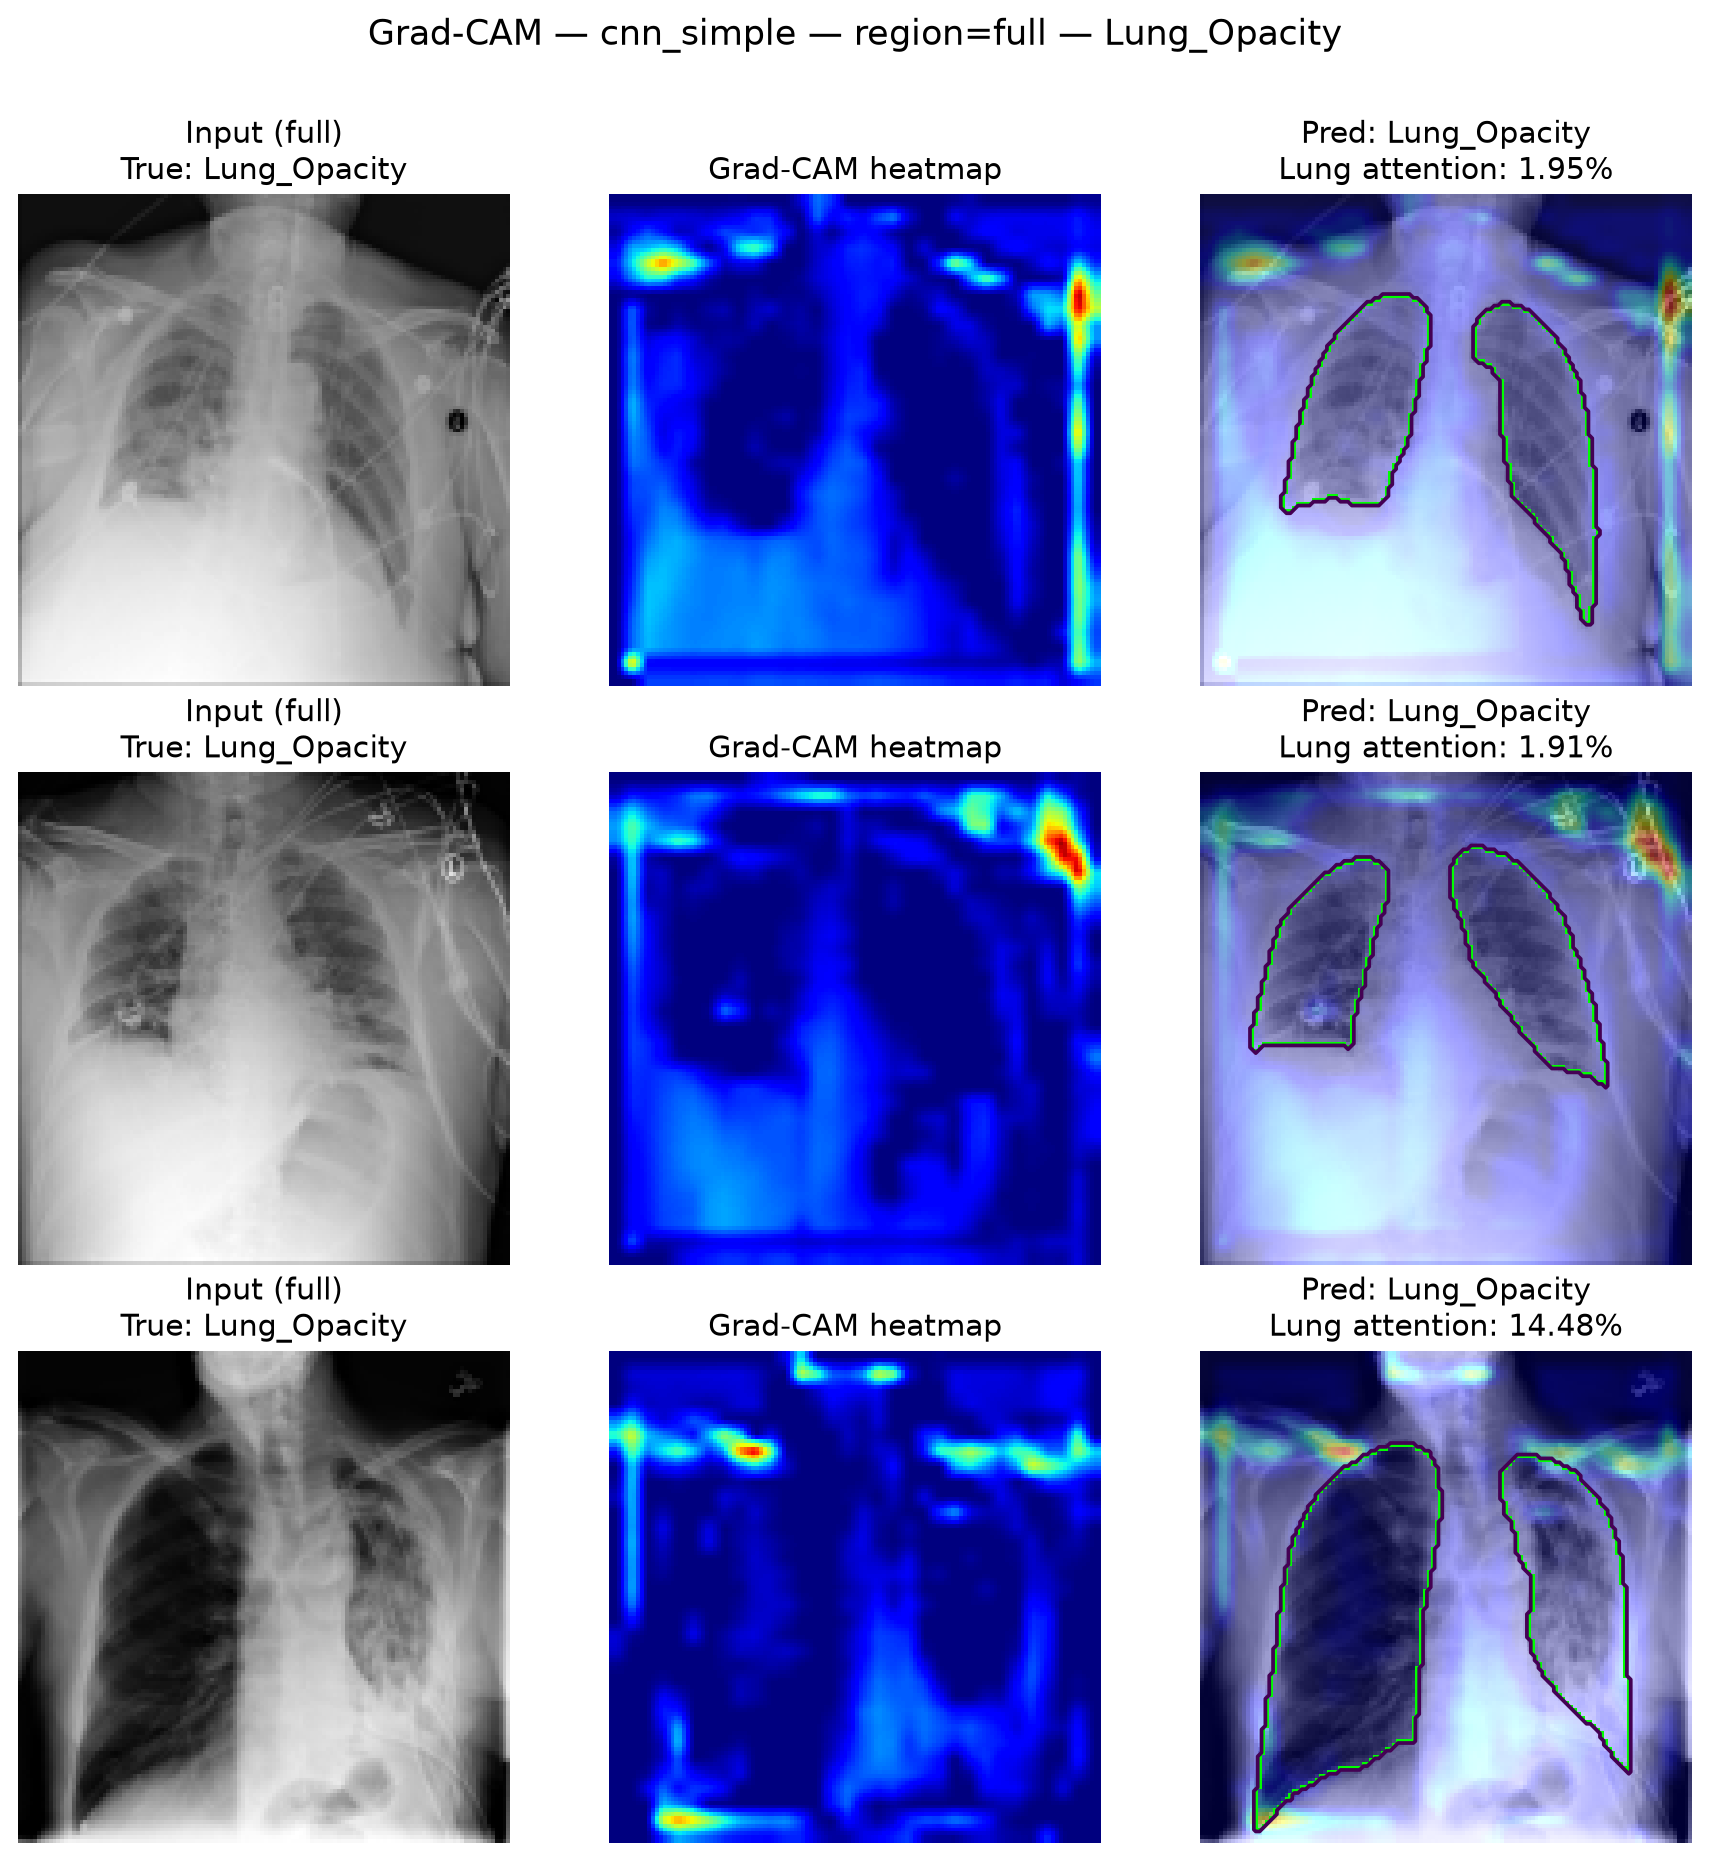
\includegraphics[width=\linewidth]{figures/gradcam_full_Lung_Opacity.png}
        \caption{Lung Opacity}
    \end{subfigure}

    \vspace{0.5em}

    \begin{subfigure}{0.48\textwidth}
        \centering
        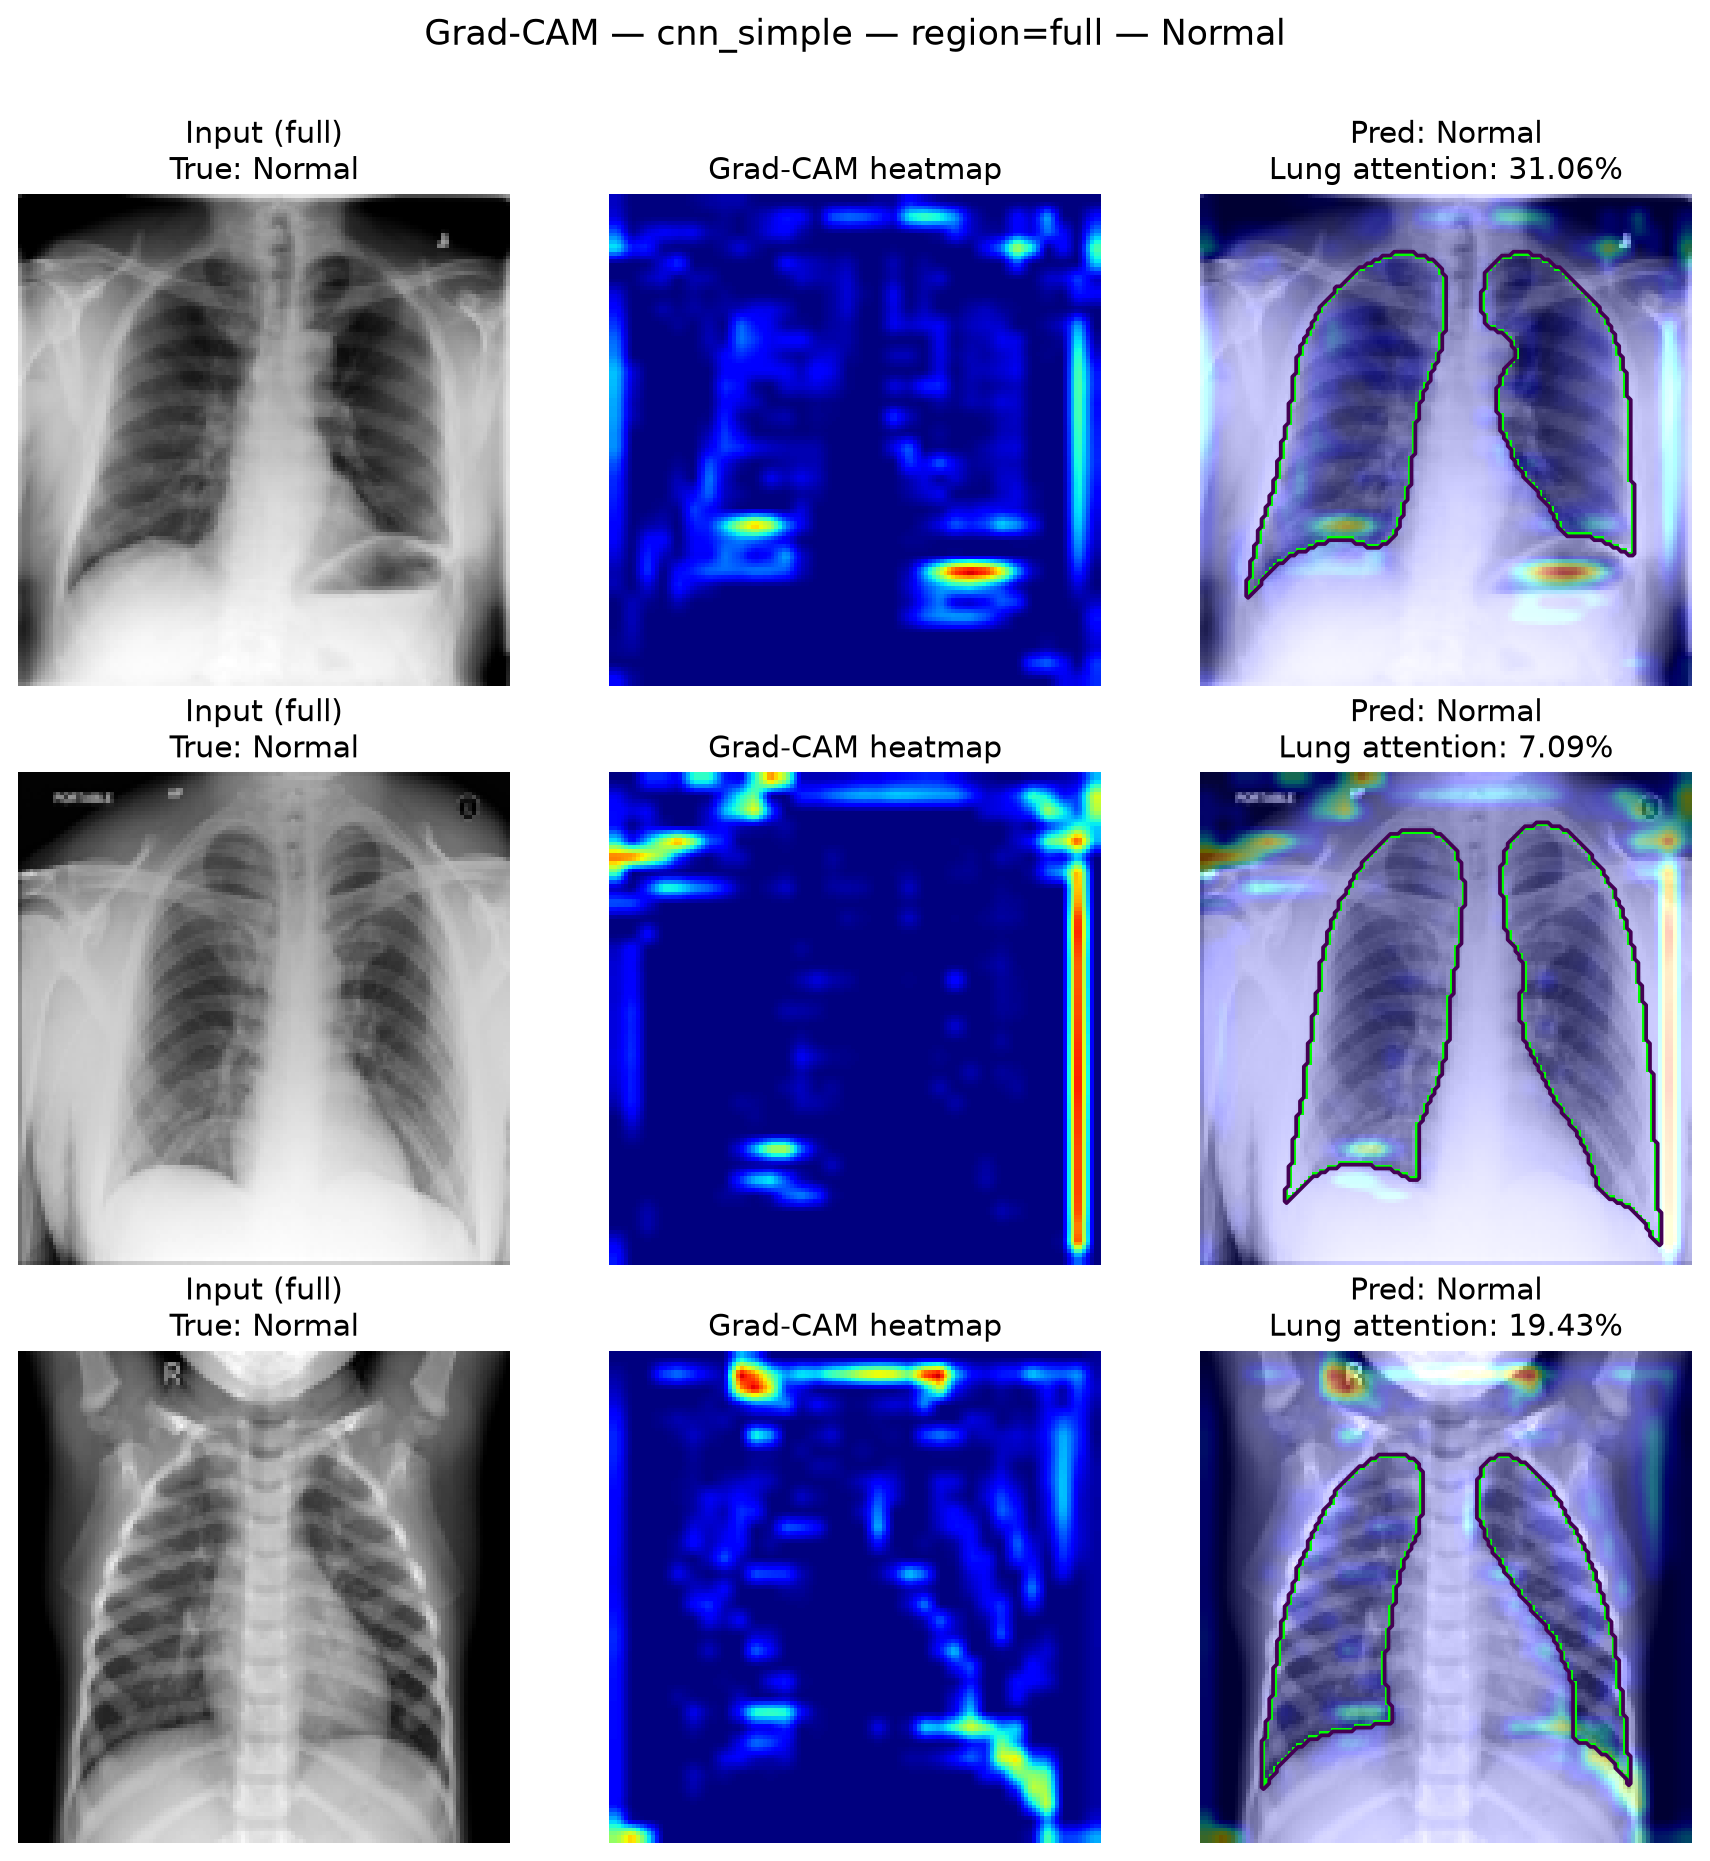
\includegraphics[width=\linewidth]{figures/gradcam_full_Normal.png}
        \caption{Normal}
    \end{subfigure}
    \hfill
    \begin{subfigure}{0.48\textwidth}
        \centering
        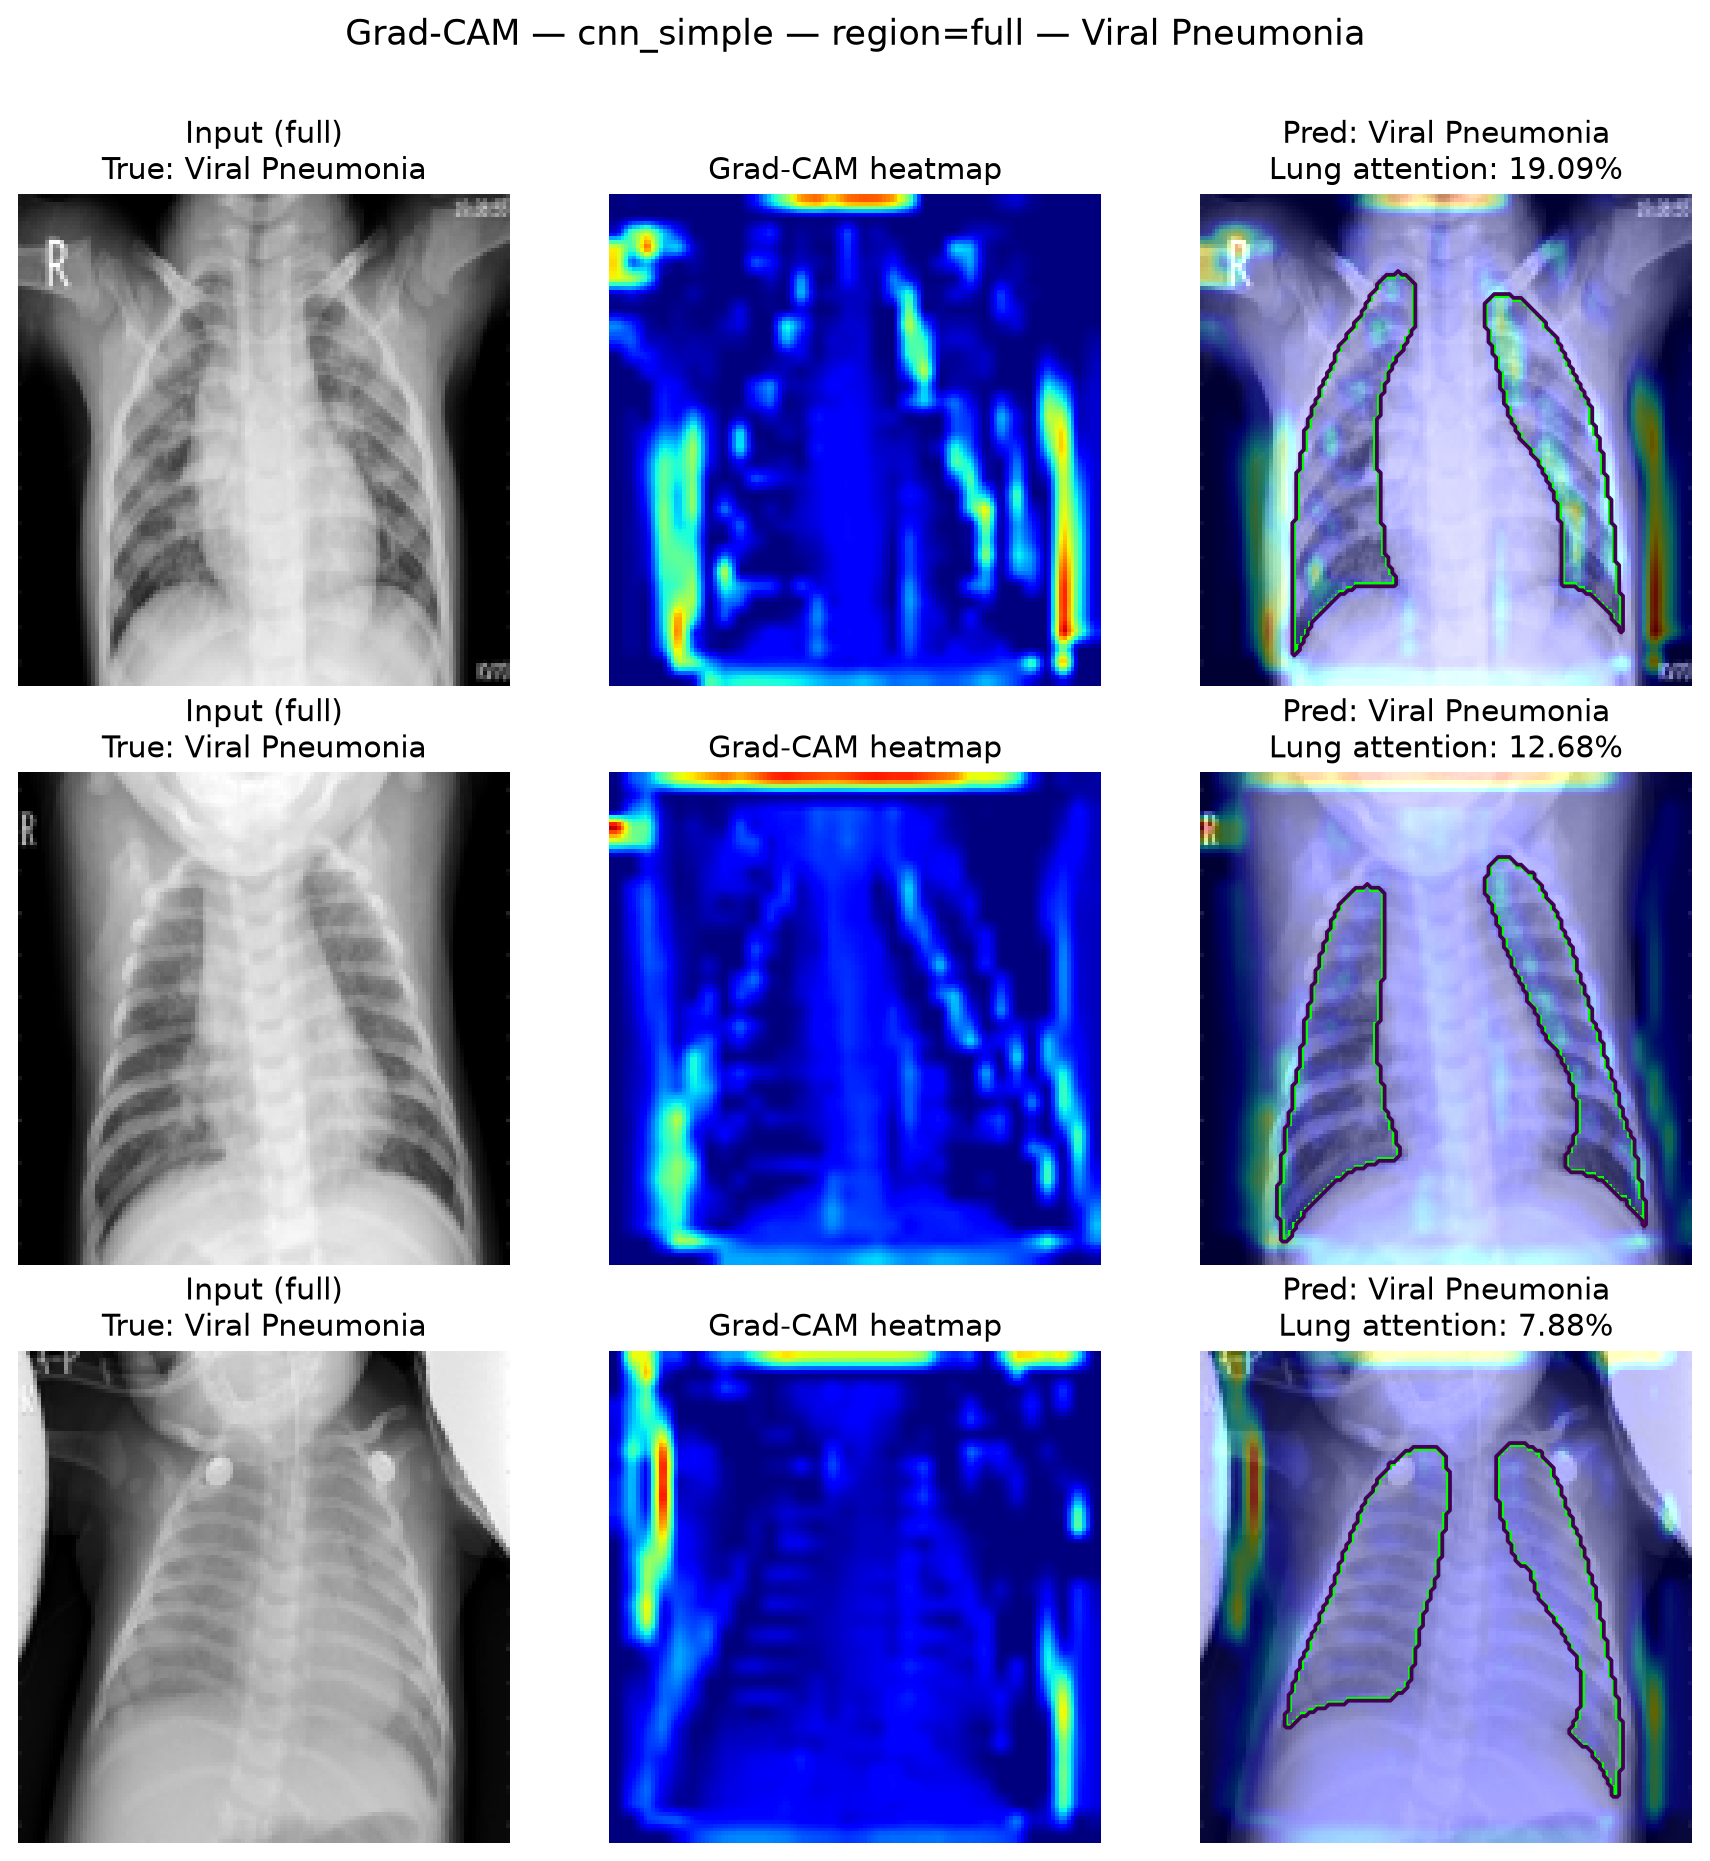
\includegraphics[width=\linewidth]{figures/gradcam_full_Viral_Pneumonia.png}
        \caption{Viral Pneumonia}
    \end{subfigure}

    \caption{Representative Grad-CAM visualisations for the lung-ROI baseline, grouped by class. Although the ROI reduces peripheral image content and avoids hard
    segmentation boundaries, model attention remains heterogeneous and is not
    restricted exclusively to the pulmonary parenchyma.}
    \label{fig:gradcam_full}
\end{figure}


\subsection{Baseline Interpretation and Role in Subsequent Experiments}
\label{subsec:baseline_role}

The two baselines provide complementary reference points for subsequent model
development.

The full-image model achieved the highest baseline performance, with 81.96\%
test accuracy and 82.7\% macro F1. However, the background-only experiment and
Grad-CAM analysis indicate that non-lung regions contain substantial
class-correlated information. Consequently, the full-image model is retained
as an unconstrained or naive performance baseline.

The lung-ROI model achieved 78.71\% test accuracy and 77.4\% macro F1 while
substantially reducing peripheral image content and avoiding the hard-mask
boundary artefact. It therefore serves as a more spatially controlled second
baseline.

These configurations will be retained when evaluating subsequent augmentation
and transfer-learning approaches. 

\if false
In particular, advanced architectures can be
compared in both input regimes:

\begin{table}[H]
\centering
\caption{Planned comparison framework for subsequent models.}
\label{tab:future_model_comparison}
\begin{tabular}{lcc}
\toprule
\textbf{Model Family} & \textbf{Full Image} & \textbf{Lung ROI} \\
\midrule
Simple CNN        & 81.96\% & 78.71\% \\
Transfer Model 1  & TBD & TBD \\
Transfer Model 2  & TBD & TBD \\
Transfer Model 3  & TBD & TBD \\
\bottomrule
\end{tabular}
\end{table}

\fi

This design supports two complementary questions:

\begin{enumerate}
    \item Does a more advanced model improve overall classification performance
    on the complete chest radiograph?
    \item Does the model also improve performance when access to obvious
    peripheral and background cues is reduced?
\end{enumerate}

The second comparison is particularly important because an improvement in
full-image accuracy alone does not necessarily imply improved use of
clinically relevant pulmonary information.